\documentclass[12pt,a4paper]{report}
\usepackage{graphicx} % Required for inserting images
\usepackage[a4paper, margin=1in]{geometry}
\usepackage{amsthm}
\usepackage{amsmath,amssymb}
\usepackage{cleveref}
\usepackage{mathtools}
\usepackage{tikz}
\usepackage{footmisc}
\usepackage{comment}
\usepackage{tikz}
\usepackage{xcolor}
\usetikzlibrary{positioning}
% --- Shrink all footnote callout marks in body text ---
\makeatletter
\renewcommand{\@makefnmark}{%
  \hbox{\textsuperscript{\normalfont\tiny\@thefnmark}}% Use \tiny or \ssmall for very small marks
}
\makeatother

% --- Optional: Set bottom footnote text size ---
\renewcommand{\footnotelayout}{\scriptsize} % Options: \scriptsize, \tiny
\renewcommand{\thefootnote}{\alph{footnote}}
\newcommand{\sidenote}[1]{\tag*{\text{\small (#1)}}}
\newcommand{\sidnote}[1]{%
  \ifmmode
    \tag*{\text{\small (#1)}}%
  \else
    \textup{(#1)}%
  \fi
}
\title{Population Dynamics(508)}
\author{MD Salauddin}
\date{September 2026}

\begin{document}

\maketitle
\tableofcontents
\newpage
\include{chapter 1/Intro1}
\section*{Dynamical System}

A system of equations:
\begin{align*}
    \frac{dx}{dt} &= P(x, y) \\
    \frac{dy}{dt} &= Q(x, y)
\end{align*}
which represents a physical problem is called a \textbf{dynamical system}.

\subsubsection*{Example:}
Consider the system of equations:
\begin{align*}
    \frac{dx}{dt} &= x - y \\
    \frac{dy}{dt} &= -x + y
\end{align*}
This is a dynamical system.
\section*{Autonomous and Non-Autonomous Dynamical Systems}

An \textbf{autonomous dynamical system} is a system of differential equations in which the independent variable time $t$ does not explicitly appear in the defining functions.

\subsection*{Formulation}
In a two-dimensional system, it is represented as:
\begin{align*}
    \dot{x} &= \frac{dx}{dt} = P(x, y) \\
    \dot{y} &= \frac{dy}{dt} = Q(x, y)
\end{align*}
where the functions $P$ and $Q$ depend solely on the state variables $x$ and $y$, and not directly on $t$.

\subsection*{Non-Autonomous Dynamical System}
If the independent variable $t$ appears explicitly in the governing equations, the system is called a \textbf{non-autonomous system}:
\begin{align*}
    \dot{x} &= \frac{dx}{dt} = P(x, y, t) \\
    \dot{y} &= \frac{dy}{dt} = Q(x, y, t)
\end{align*}

\subsection*{Examples}

\subsubsection*{1. Autonomous System:}
\begin{align*}
    \dot{x} &= xy \\
    \dot{y} &= x^2 + y^2
\end{align*}
\noindent \textit{(No explicit time parameter $t$ on the right-hand side.)}

\subsubsection*{2. Non-Autonomous System:}
\begin{align*}
    \dot{x} &= xt + y \\
    \dot{y} &= x^2 + y^2 + t^2
\end{align*}
\noindent \textit{(Time parameter $t$ explicitly appears on the right-hand side.)}
\section*{Critical Point}

Let
\begin{equation}
    \dot{x} = P(x, y), \quad \dot{y} = Q(x, y) \sidenote{1}
\end{equation}
be a dynamical system. A point $(x_0, y_0)$ is called a \textbf{critical point} of the system (1) if:

\begin{enumerate}
    \item[(i)] $P(x_0, y_0) = 0$ \quad \text{and} \quad $Q(x_0, y_0) = 0$
\end{enumerate}

\noindent i.e.,
\begin{align*}
    \dot{x} &= 0 \\
    \dot{y} &= 0
\end{align*}

\section*{Isolated Critical Points}

Let
\begin{equation}
    \dot{x} = P(x, y) \quad \text{and} \quad \dot{y} = Q(x, y) \sidenote{i}
\end{equation}
be a dynamical system, and let $(x_0, y_0)$ be a critical point of (i). If there exists a neighborhood of the critical point $(x_0, y_0)$ such that no other critical point lies in that neighborhood, then $(x_0, y_0)$ is called an \textbf{isolated critical point}.

\vspace{0.5em}
\noindent There are four types of isolated critical points:
\begin{enumerate}
    \item[(i)] Node
    \item[(ii)] Saddle point
    \item[(iii)] Spiral (Focus)
    \item[(iv)] Center
\end{enumerate}
\section*{Node:}
Consider the autonomous dynamical system:
\[
\dot{x} = P(x, y), \quad \dot{y} = Q(x, y)
\]
with an isolated critical point at the origin $(0, 0)$. The critical point $(0, 0)$ is called a \textbf{node} if:

\begin{enumerate}
    \item Every trajectory in a neighborhood of $(0, 0)$ approaches $(0, 0)$ either as $t \to +\infty$ (stable node) or as $t \to -\infty$ (unstable node).
    \item Every trajectory enters or leaves $(0, 0)$ along a \textbf{well-defined tangent line} (a definite direction).
    \item Trajectories \textbf{do not spiral or rotate} infinitely around $(0, 0)$ as they approach or leave it.
\end{enumerate}

\subsection*{Alternative (Eigenvalue Criterion for Linear Systems)}

If the condition is given in terms of linear system dynamics ($\dot{\mathbf{x}} = A\mathbf{x}$):

\begin{quote}
\textit{The isolated critical point $(0, 0)$ is a \textbf{node} if the eigenvalues $\lambda_1, \lambda_2$ of the Jacobian matrix evaluated at $(0, 0)$ are \textbf{real, non-zero, distinct (or proper)}, and have the same sign:}
\begin{itemize}
    \item \textbf{Stable Node:} $\lambda_1, \lambda_2 < 0$ \textit{(Real and both negative)}
    \item \textbf{Unstable Node:} $\lambda_1, \lambda_2 > 0$ \textit{(Real and both positive)}
\end{itemize}
\end{quote}
\begin{center}
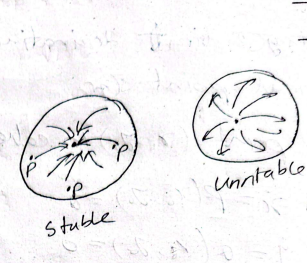
\includegraphics[width=0.6\textwidth]{Image/node.png}
\end{center}

\section*{Definition of a Saddle Point}

Consider the autonomous dynamical system $\dot{x} = P(x, y), \, \dot{y} = Q(x, y)$ with an isolated critical point at $(0, 0)$.

\vspace{0.5em}
\noindent The critical point $(0, 0)$ is called a \textbf{saddle point} if:

\begin{enumerate}
    \item There exist exactly \textbf{two trajectories} (separatrices) that approach and enter $(0, 0)$ as $t \to +\infty$ from opposite directions, and \textbf{two trajectories} that enter $(0, 0)$ as $t \to -\infty$ (move away as $t \to +\infty$) from opposite directions.
    \item All other trajectories in the neighborhood of $(0, 0)$ pass near the critical point without entering it and subsequently move away as $t \to \pm\infty$ (forming hyperbolic-like curves).
\end{enumerate}

\subsection*{Eigenvalue Condition (Linear Analysis)}

For the linearized system $\dot{\mathbf{x}} = A\mathbf{x}$, $(0, 0)$ is a \textbf{saddle point} if and only if the eigenvalues $\lambda_1, \lambda_2$ of the Jacobian matrix evaluated at $(0, 0)$ are \textbf{real, non-zero, and have opposite signs}:

\[
\lambda_1 < 0 < \lambda_2 \quad \text{(or } \det(A) < 0\text{)}
\]
\begin{center}
    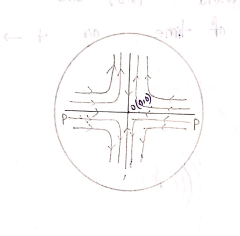
\includegraphics[width=0.5\textwidth]{Image/saddle point.png}
\end{center}
\section*{Definition of a Spiral (or Focus)}

Consider the autonomous dynamical system $\dot{x} = P(x, y), \, \dot{y} = Q(x, y)$ with an isolated critical point at $(0, 0)$.

\vspace{0.5em}
\noindent The critical point $(0, 0)$ is called a \textbf{spiral} (or \textbf{focus}) if:

\begin{enumerate}
    \item Trajectories starting at any point $P$ in a neighborhood of $(0, 0)$ approach the origin as $t \to +\infty$ (stable spiral) or move away from the origin as $t \to +\infty$ (unstable spiral).
    \item Trajectories wind around $(0, 0)$ \textbf{infinitely many times} in a spiral-like manner as they approach or move away from the critical point.
    \item Trajectories \textbf{do not enter or leave along a single well-defined tangent line}, as the direction angle $\theta(t) \to \pm\infty$.
\end{enumerate}

\subsection*{Eigenvalue Condition (Linear Analysis)}

For the linearized system $\dot{\mathbf{x}} = A\mathbf{x}$, $(0, 0)$ is a \textbf{spiral point} if and only if the eigenvalues $\lambda_1, \lambda_2$ of the Jacobian matrix $A$ evaluated at $(0, 0)$ are \textbf{complex conjugates with a non-zero real part}:

\[
\lambda_{1,2} = \alpha \pm i\beta, \quad \text{where } \alpha \neq 0 \text{ and } \beta \neq 0
\]

\begin{itemize}
    \item \textbf{Stable Spiral (Sink):} $\alpha = \text{Re}(\lambda) < 0$ \textit{(trajectories spiral inward toward $(0, 0)$)}.
    \item \textbf{Unstable Spiral (Source):} $\alpha = \text{Re}(\lambda) > 0$ \textit{(trajectories spiral outward away from $(0, 0)$)}.
\end{itemize}
\begin{center}
    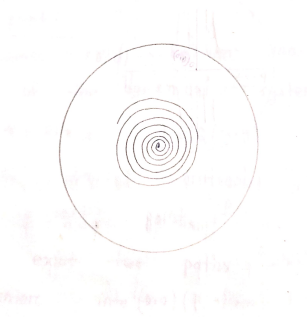
\includegraphics[width=0.5 \textwidth]{Image/spiral.png}
\end{center}
\section*{Definition of a Center}

Consider the autonomous dynamical system $\dot{x} = P(x, y), \, \dot{y} = Q(x, y)$ with an isolated critical point at $(0, 0)$.

\vspace{0.5em}
\noindent The critical point $(0, 0)$ is called a \textbf{center} (or \textbf{centre}) if:

\begin{enumerate}
    \item Every neighborhood of $(0, 0)$ contains a family of \textbf{closed concentric trajectories} (ellipses or circles) enclosing $(0, 0)$ as an interior point.
    \item Trajectories around $(0, 0)$ are periodic and closed, meaning they \textbf{neither approach nor move away} from $(0, 0)$ as $t \to \pm\infty$.
\end{enumerate}

\subsection*{Eigenvalue Condition (Linear Analysis)}

For the linearized system $\dot{\mathbf{x}} = A\mathbf{x}$, $(0, 0)$ is a \textbf{center} if and only if the eigenvalues $\lambda_1, \lambda_2$ of the Jacobian matrix $A$ evaluated at $(0, 0)$ are \textbf{purely imaginary}:

\[
\lambda_{1,2} = \pm i\omega \quad (\text{where } \omega \in \mathbb{R}, \, \omega \neq 0)
\]
\begin{center}
    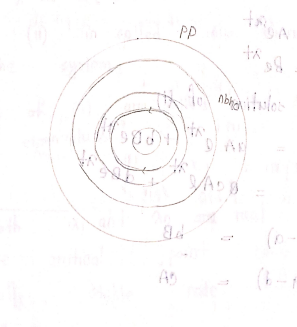
\includegraphics[width=0.4 \textwidth]{Image/center.png}
\end{center}
\chapter{Periodic solutions}
\section*{Info}
\begin{itemize}
    \item Green's Theorem\\
    Let $C$ be a positively oriented (counterclockwise), piecewise-smooth, simple closed curve in the $xy$-plane, and let $D$ be the region bounded by $C$.If $P(x, y)$ and $Q(x, y)$ are functions that have continuous first-order partial derivatives ($\frac{\partial P}{\partial y}$ and $\frac{\partial Q}{\partial x}$) on an open region containing $D$, then: Line Integral / Double Integral Form (Standard Form)$$\oint_C (P \, dx + Q \, dy) = \iint_D \left( \frac{\partial Q}{\partial x} - \frac{\partial P}{\partial y} \right) dA$$where $dA = dx \, dy$ (or $dy \, dx$).
    \item \textbf{Angular equation:}
\[
r^2 \dot{\theta} = x\dot{y} - y\dot{x}
\]
\end{itemize}
\section*{Closed Path}

If the initial and terminal points of a path are identical, then the path is called a \textbf{closed path}.

\vspace{0.5em}
\noindent \textbf{Examples of Closed Paths:}
\begin{itemize}
    \item A circle or ellipse returning to its starting point.
\end{itemize}

\section*{ Non-Closed Path}

If the initial and terminal points of a path are not identical, then the path is called a \textbf{non-closed path} (or open path).

\vspace{0.5em}
\noindent \textbf{Example of a Non-Closed Path:}
\begin{itemize}
    \item An open curve or line segment where the start and end points do not coincide.
\end{itemize}
\section*{Periodic Solution}

Consider the dynamical system:
\begin{equation}
    \begin{aligned}
        \dot{x} &= P(x, y) \\
        \dot{y} &= Q(x, y)
    \end{aligned} \sidenote{1}
\end{equation}

\noindent Let $x = f(t)$ and $y = g(t)$ be a solution of system (1). Then the solution is called a \textbf{periodic solution} if there exists a constant $T > 0$ such that:
\[
f(t + T) = f(t) \quad \text{and} \quad g(t + T) = g(t) \quad \text{for all } t
\]

\noindent Here, $T$ is called the \textbf{period} of the solution.
\section*{Limit Cycle}

A closed path $C$ of a system:
\begin{equation}
    \begin{aligned}
        \dot{x} &= P(x, y) \\
        \dot{y} &= Q(x, y)
    \end{aligned} \sidenote{1}
\end{equation}

\noindent which is approached spirally from either inside or outside by a non-closed path $C_1$ of system (1) as $t \to +\infty$ or $t \to -\infty$ is called a \textbf{limit cycle} of the system (1).
\begin{center}
    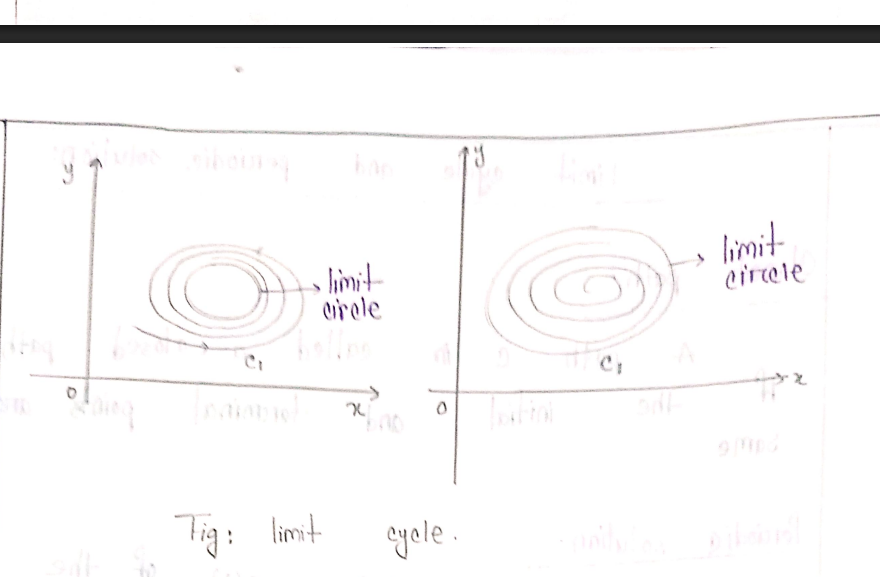
\includegraphics[width=0.5 \textwidth]{Image/limit cycle.png}
\end{center}
\section{State and prove Bendixon's non-existence theorem.}
\subsection*{Statement}

If $P(x, y)$ and $Q(x, y)$ of the system:
\begin{equation}
    \begin{aligned}
        \dot{x} &= P(x, y) \\
        \dot{y} &= Q(x, y)
    \end{aligned} \sidenote{1}
\end{equation}
have continuous first-order partial derivatives in a simply-connected domain $D$ of the $xy$-plane, and if $\frac{\partial P}{\partial x} + \frac{\partial Q}{\partial y}$
has the same sign throughout $D$, then system (1) has no closed path (periodic solution) in $D$.
\subsection*{Proof}
Let $C$ be a closed path in $D$ and $R$ be the region bounded by $C$.

\noindent Then by Green's theorem in the plane, we have:
\begin{equation}
    \oint_C \left[ P(x, y) \, dy - Q(x, y) \, dx \right] = \iint_R \left[ \frac{\partial P(x, y)}{\partial x} + \frac{\partial Q(x, y)}{\partial y} \right] dx \, dy \sidenote{2}
\end{equation}
where the line integral is taken in the positive (counterclockwise) sense.

\vspace{0.5em}
\noindent Now, assume that $C$ is a closed path of system (1).

\noindent Let $x = f(t), \, y = g(t)$ be a periodic solution of system (1) representing the closed path $C$ with period $T$.

\noindent Along the trajectory $C$:
\begin{equation}
    \begin{aligned}
        \dot{x} &= \frac{dx}{dt} = \frac{df(t)}{dt} = P(x, y) = P(f(t), g(t)) \\
        \dot{y} &= \frac{dy}{dt} = \frac{dg(t)}{dt} = Q(x, y) = Q(f(t), g(t))
    \end{aligned} \sidenote{3}
\end{equation}

\noindent Substituting (3) into the Left-Hand Side (L.H.S.) of equation (2):
\begin{align*}
    \text{L.H.S. of (2)} &= \oint_C \left[ P(x, y) \, dy - Q(x, y) \, dx \right] \\[0.5em]
    &= \int_0^T \left[ P(f(t), g(t)) \frac{dg}{dt} - Q(f(t), g(t)) \frac{df}{dt} \right] dt \\[0.5em]
    &= \int_0^T \left[ P(f(t), g(t)) \cdot Q(f(t), g(t)) - Q(f(t), g(t)) \cdot P(f(t), g(t)) \right] dt \quad \text{[Using (3)]} \\[0.5em]
    &= 0
\end{align*}

\noindent Substituting this result back into equation (2) yields:
\begin{equation}
    \iint_R \left( \frac{\partial P}{\partial x} + \frac{\partial Q}{\partial y} \right) dx \, dy = 0 \sidenote{4}
\end{equation}
But this double integral can be zero only if $\left( \frac{\partial P}{\partial x} + \frac{\partial Q}{\partial y} \right)$ changes sign in $R$.This is a contradiction.Thus, $C$ is not a path of system (i). Hence, the system (i) has no closed path or periodic solution in $D$.
\section{Examine the existence of limit cycle and periodic solution of the system:If periodic solutions exist, find them and sketch the phase portrait.}
$$\dot{x} = -y + x(1 - x^2 - y^2)$$$$\dot{y} = x + y(1 - x^2 - y^2)$$
\subsection*{Solution:}
Consider the non-linear autonomous dynamical system:
\begin{align*}
    \dot{x} &= -y + x(1 - x^2 - y^2)=P(x,y) \\
    \dot{y} &= x + y(1 - x^2 - y^2)=Q(x,y)
\end{align*}
now, $P(x, y) = -y + x(1 - x^2 - y^2)$ and $Q(x, y) = x + y(1 - x^2 - y^2)$.

\noindent Computing partial derivatives:
\[
\frac{\partial P}{\partial x} = (1 - x^2 - y^2) + x(-2x) = 1 - 3x^2 - y^2
\]
\[
\frac{\partial Q}{\partial y} = (1 - x^2 - y^2) + y(-2y) = 1 - x^2 - 3y^2
\]

\noindent Calculating the divergence of the vector field:
\[
\nabla \cdot \mathbf{f} = \frac{\partial P}{\partial x} + \frac{\partial Q}{\partial y} = 2 - 4x^2 - 4y^2 = 2 \left[ 1 - 2(x^2 + y^2) \right]
\]

\noindent Since $\frac{\partial P}{\partial x} + \frac{\partial Q}{\partial y}$ changes sign, Bendixson's negative criterion does not rule out the existence of closed trajectories.
Using the transformation $x = r \cos\theta$ and $y = r \sin\theta$, where $r^2 = x^2 + y^2$:
Differentiating $r^2 = x^2 + y^2$ with respect to $t$:
\[
2r\dot{r} = 2x\dot{x} + 2y\dot{y} \implies r\dot{r} = x\dot{x} + y\dot{y}
\]
Substituting $\dot{x}$ and $\dot{y}$:
\begin{align*}
    x\dot{x} + y\dot{y} &= x \left[ -y + x(1 - r^2) \right] + y \left[ x + y(1 - r^2) \right] \\
    &= -xy + x^2(1 - r^2) + xy + y^2(1 - r^2) \\
    &= (x^2 + y^2)(1 - r^2) = r^2(1 - r^2)
\end{align*}
Equating $r\dot{r} = r^2(1 - r^2)$ (for $r \neq 0$):
\[
\dot{r} = r(1 - r^2)
\]

\subsubsection*{ Angular Equation ($\dot{\theta}$)}
Using $r^2 \dot{\theta} = x\dot{y} - y\dot{x}$:
\begin{align*}
    x\dot{y} - y\dot{x} &= x \left[ x + y(1 - r^2) \right] - y \left[ -y + x(1 - r^2) \right] \\
    &= x^2 + xy(1 - r^2) + y^2 - xy(1 - r^2) \\
    &= x^2 + y^2 = r^2
\end{align*}
Equating $r^2 \dot{\theta} = r^2$:
\[
\dot{\theta} = 1
\]
\[
\frac{d\theta}{dt} = 1 \implies \theta(t) = t + \theta_0
\]
Setting phase angle $\theta_0 = 0$ for simplicity gives $\theta(t) = t$.

Separating variables in $\frac{dr}{dt} = r(1 - r^2)$:
\[
\frac{dr}{r(1 - r^2)} = dt
\]
Applying partial fraction decomposition:
\[
\int \left( \frac{1}{r} + \frac{r}{1 - r^2} \right) dr = \int dt
\]
\[
\ln r - \frac{1}{2}\ln|1 - r^2| = t + k
\]
\[
\ln \left( \frac{r}{\sqrt{|1 - r^2|}} \right) = t + k \implies \frac{r^2}{|1 - r^2|} = C_1 e^{2t} \quad (C_1 = e^{2k})
\]
Solving for $r^2$:
\[
r^2 = \frac{C_0 e^{2t}}{1 + C_0 e^{2t}} = \frac{1}{1 + C e^{-2t}} \quad \left( C = \frac{1}{C_0} \right)
\]
With initial condition $r(0) = r_0$, we obtain $C = \frac{1 - r_0^2}{r_0^2}$:
\[
r(t) = \frac{1}{\sqrt{1 + \left( \frac{1 - r_0^2}{r_0^2} \right) e^{-2t}}}
\]
\begin{align*}
    \therefore x(t) &= r(t)\cos(t) = \frac{\cos t}{\sqrt{1 + \left( \frac{1 - r_0^2}{r_0^2} \right) e^{-2t}}} \\[0.5em]
    \text{and} y(t) &= r(t)\sin(t) = \frac{\sin t}{\sqrt{1 + \left( \frac{1 - r_0^2}{r_0^2} \right) e^{-2t}}}
\end{align*}
\begin{enumerate}
    \item \textbf{Periodic Orbit / Limit Cycle ($r_0 = 1$):} \\
    If $r_0 = 1$, then $r(t) = 1$ for all $t \ge 0$. The solution simplifies to:
    \[
    x(t) = \cos t, \quad y(t) = \sin t
    \]
    This represents an isolated closed trajectory (a circle of radius $r = 1$) in the phase plane.

    \item \textbf{Outer Trajectories ($r_0 > 1$):} \\
    As $t \to +\infty$, $e^{-2t} \to 0$, which yields $r(t) \to 1^-$. Trajectories starting outside the unit circle spiral inward toward $r = 1$.

    \item \textbf{Inner Trajectories ($0 < r_0 < 1$):} \\
    As $t \to +\infty$, $e^{-2t} \to 0$, which yields $r(t) \to 1^+$. Trajectories starting inside the unit circle spiral outward toward $r = 1$.
\end{enumerate}

\noindent \textbf{Conclusion:} Because all nearby trajectories approach $r = 1$ as $t \to +\infty$ from both interior and exterior regions, $r = 1$ is a \textbf{stable limit cycle}.
\begin{center}
    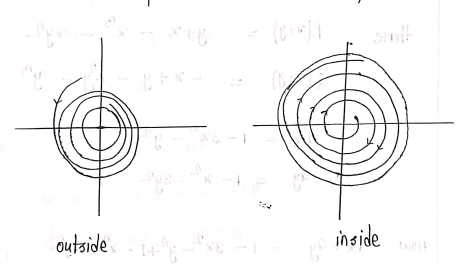
\includegraphics[]{Image/phase portrait 1.png}
\end{center}
\section{Problem: Existence of a Limit Cycle for the system:\textcolor{green}{2021} }
\begin{align*}
    \dot{x} &= 4x - 4y - x(x^2 + y^2) \\
    \dot{y} &= 4x + 4y - y(x^2 + y^2)
\end{align*}
and verify that $x = 2\cos(4t)$, $y = 2\sin(4t)$ is a periodic solution of this system.

\bigskip
\noindent \textbf{Solution:}

Given system of differential equations:
\begin{align*}
    \dot{x} &= 4x - 4y - x(x^2 + y^2) \tag{1a} \\
    \dot{y} &= 4x + 4y - y(x^2 + y^2) \tag{1b}
\end{align*}

Let $P(x, y) = 4x - 4y - x(x^2 + y^2)$ and $Q(x, y) = 4x + 4y - y(x^2 + y^2)$.

Computing partial derivatives:
\begin{align*}
    \frac{\partial P}{\partial x} &= 4 - 3x^2 - y^2 \\
    \frac{\partial Q}{\partial y} &= 4 - x^2 - 3y^2
\end{align*}

Taking the sum (divergence of the vector field):
\begin{align*}
    \frac{\partial P}{\partial x} + \frac{\partial Q}{\partial y} &= (4 - 3x^2 - y^2) + (4 - x^2 - 3y^2) \\
    &= 8 - 4(x^2 + y^2) \sidenote{divergence changes sign at $r = \sqrt{2}$}
\end{align*}

Since $\frac{\partial P}{\partial x} + \frac{\partial Q}{\partial y}$ changes sign in the plane, Bendixson's criterion does not rule out periodic orbits. Thus, the system admits a limit cycle.

\bigskip
\noindent \textbf{Verification of Periodic Solution:}

Given proposed solution:
\begin{align*}
    x(t) &= 2\cos(4t) \tag{a} \\
    y(t) &= 2\sin(4t)
\end{align*}

Differentiating with respect to $t$:
\begin{align*}
    \dot{x} &= -8\sin(4t) \tag{b} \\
    \dot{y} &= 8\cos(4t)
\end{align*}

Substituting (a) into the right-hand side of equation (1a):
\begin{align*}
    \text{RHS} &= 4(2\cos 4t) - 4(2\sin 4t) - 2\cos 4t \left(4\cos^2 4t + 4\sin^2 4t\right) \sidenote{$x^2+y^2 = 4$} \\
    &= 8\cos 4t - 8\sin 4t - 2\cos 4t (4) \\
    &= -8\sin 4t = \dot{x}
     \text{RHS}\\ &= 4(2\cos 4t) + 4(2\sin 4t) - 2\sin 4t \left(4\cos^2 4t + 4\sin^2 4t\right) \\
    &= 8\cos 4t + 8\sin 4t - 2\sin 4t (4) \\
    &= 8\cos 4t = \dot{y}
\end{align*}
Hence, $x(t) = 2\cos(4t), y(t) = 2\sin(4t)$ is a periodic solution of the system.\\
\textit{There are two math problems in page around 110 on periodic solution, you should look on it.}
\chapter{Stability Theorem}
\section*{ABC}
\begin{itemize}
    \item positive definite
    \item Positive semi-definite
    \item Negative definite
    \item Negative semi-definite
    \item Liapunov function
    \item Trivial solution
    \item system of a non linear equation
    \section*{Poincaré–Liapunov Theorem on Linearization}

\subsection*{Statement}

Let the non-linear autonomous system be given by:
\begin{equation}
    \begin{aligned}
        \dot{x} &= ax + by + P(x, y) \\
        \dot{y} &= cx + dy + Q(x, y)
    \end{aligned} \sidenote{1}
\end{equation}

If $P(x, y)$ and $Q(x, y)$ are continuous in a neighborhood of the origin $(0,0)$ and satisfy the conditions:
\begin{align*}
    \lim_{(x, y) \to (0,0)} \frac{P(x, y)}{\sqrt{x^2 + y^2}} &= 0 \\[0.5em]
    \lim_{(x, y) \to (0,0)} \frac{Q(x, y)}{\sqrt{x^2 + y^2}} &= 0
\end{align*}

then the characteristic nature and qualitative stability of the critical point at the origin $(0,0)$ for the non-linear system (1) is the same as that of the corresponding linearized system:
\item Squeez Theorem:\\
Let $f(x, y)$, $g(x, y)$, and $h(x, y)$ be functions defined on a neighborhood of $(x_0, y_0)$, except possibly at $(x_0, y_0)$ itself.If for all $(x, y) \neq (x_0, y_0)$ in that neighborhood:$$g(x, y) \le f(x, y) \le h(x, y)$$and if:$$\lim_{(x,y) \to (x_0, y_0)} g(x, y) = L \quad \text{and} \quad \lim_{(x,y) \to (x_0, y_0)} h(x, y) = L$$then:$$\lim_{(x,y) \to (x_0, y_0)} f(x, y) = L$$
For example:\\
$$\left\vert{} \frac{-x^2}{\sqrt{x^2 + y^2}} \right\vert{} = \frac{\vert{}x\vert{} \cdot \vert{}x\vert{}}{\sqrt{x^2 + y^2}} \le \frac{\vert{}x\vert{} \cdot \sqrt{x^2 + y^2}}{\sqrt{x^2 + y^2}} = \vert{}x\vert{} \left[\vert{}x\vert{} \le \sqrt{x^2+y^2}\right]$$Thus:$$0 \le \left\vert{} \frac{-x^2}{\sqrt{x^2 + y^2}} \right\vert{} \le \vert{}x\vert{}$$Taking the limit as $(x,y) \to (0,0)$:$$\lim_{(x,y) \to (0,0)} 0 = 0 \quad \text{and} \quad \lim_{(x,y) \to (0,0)} \vert{}x\vert{} = 0$$By the Squeeze Theorem:$$\lim_{(x,y) \to (0,0)} \frac{-x^2}{\sqrt{x^2 + y^2}} = 0$$
\end{itemize}

\section{The given system ,Test whether the system stable or unstable}
\begin{align*}
    \dot{x}&=ax+by\\
    \dot{y} &=cx+dy
\end{align*}
\section*{Solution}
Consider the two-dimensional linear homogeneous autonomous system:
\begin{equation}
    \begin{aligned}
        \dot{x} &= ax + by \\
        \dot{y} &= cx + dy
    \end{aligned} \sidenote{1}
\end{equation}
Assume a trial solution of the form:
\[
x(t) = A e^{\lambda t}, \quad y(t) = B e^{\lambda t}
\]
where $A$ and $B$ are non-zero constants.

\noindent Differentiating and substituting into system (1):
\begin{align*}
    A \lambda e^{\lambda t} &= a A e^{\lambda t} + b B e^{\lambda t} \\
    B \lambda e^{\lambda t} &= c A e^{\lambda t} + d B e^{\lambda t}
\end{align*}

\noindent Since $e^{\lambda t} \neq 0$ for all $t$:
\begin{align*}
    A \lambda &= a A + b B \\
    B \lambda &= c A + d B
\end{align*}

\noindent Rearranging into a homogeneous linear system:
\begin{align*}
    (\lambda - a)A - b B &= 0 \\
    -cA + (\lambda - d)B &= 0
\end{align*}

\noindent For non-trivial solutions $(A, B) \neq (0, 0)$, the determinant of the coefficient matrix must vanish:
\[
\begin{vmatrix}
\lambda - a & -b \\
-c & \lambda - d
\end{vmatrix} = 0
\]

\noindent Expanding the determinant:
\[
(\lambda - a)(\lambda - d) - bc = 0
\]
\[
\lambda^2 - (a + d)\lambda + (ad - bc) = 0
\]

\noindent Solving using the quadratic formula:
\[
\lambda_{1,2} = \frac{(a + d) \pm \sqrt{(a + d)^2 - 4(ad - bc)}}{2}
\]
\[
\lambda_{1,2} = \frac{(a + d) \pm \sqrt{(a - d)^2 + 4bc}}{2}
\]

\subsection*{Classification of Critical Points (Origin)}

\begin{enumerate}
    \item \textbf{Stable Node:} If $\lambda_1$ and $\lambda_2$ are real, distinct, and both negative ($\lambda_1 < \lambda_2 < 0$), the system at the origin is a \textbf{stable node}.
    
    \item \textbf{Unstable Node:} If $\lambda_1$ and $\lambda_2$ are real, distinct, and both positive ($\lambda_1 > \lambda_2 > 0$), the system at the origin is an \textbf{unstable node}.
    
    \item \textbf{Stable Center:} If $\lambda_1$ and $\lambda_2$ are purely imaginary ($\lambda_{1,2} = \pm i\beta$), the system at the origin is a \textbf{stable center} (neutrally stable).
    
    \item \textbf{Unstable Spiral:} If $\lambda_1$ and $\lambda_2$ are complex conjugates with positive real part ($\lambda_{1,2} = \alpha \pm i\beta, \; \alpha > 0$), the system at the origin is an \textbf{unstable spiral (focus)}.
    
    \item \textbf{Stable Spiral:} If $\lambda_1$ and $\lambda_2$ are complex conjugates with negative real part ($\lambda_{1,2} = \alpha \pm i\beta, \; \alpha < 0$), the system at the origin is a \textbf{stable spiral (focus)}.
    
    \item \textbf{Unstable Saddle Point:} If one eigenvalue is positive(real) and the other is negative ($\lambda_1 < 0 < \lambda_2$), the system at the origin is an \textbf{unstable saddle point}.
\end{enumerate}
\section{Discuss the stability and nature of the critical point.}
\begin{align*}
        \dot{x} &= x + 3y \\
        \dot{y} &= 3x + y
    \end{align*}
Consider the linear autonomous dynamical system:
\begin{equation}
    \begin{aligned}
        \dot{x} &= x + 3y \\
        \dot{y} &= 3x + y
    \end{aligned} \sidenote{1}
\end{equation}

Here, the system matrix coefficients are:
\[
a = 1, \quad b = 3, \quad c = 3, \quad d = 1
\]
The characteristic equation of system (1) is given by:
\[
\lambda^2 - (a + d)\lambda + (ad - bc) = 0
\]

\noindent Substituting the values of $a, b, c,$ and $d$:
\begin{align*}
    \lambda^2 - \lambda(1 + 1) + (1 \cdot 1 - 3 \cdot 3) &= 0 \\[0.5em]
    \lambda^2 - 2\lambda - 8 &= 0 \\[0.5em]
    \lambda^2 - 4\lambda + 2\lambda - 8 &= 0 \\[0.5em]
    \lambda(\lambda - 4) + 2(\lambda - 4) &= 0 \\[0.5em]
    (\lambda - 4)(\lambda + 2) &= 0
\end{align*}

\noindent Thus, the eigenvalues are:
\[
\lambda_1 = 4, \quad \lambda_2 = -2
\]
Since one eigenvalue is real and positive ($\lambda_1 = 4 > 0$) and the other eigenvalue is real and negative ($\lambda_2 = -2 < 0$), the critical point at the origin $(0, 0)$ is an \textbf{unstable saddle point}.
\section{Discuss the stability and nature of the critical point of the non linear system and sketch the phase portrait.}
\begin{align*}
        \dot{x} &= x + 4y - x^2 \\
        \dot{y} &= 6x - y + 2xy
    \end{align*}
\subsection*{Solution}

Given the non-linear system:
\begin{equation}
    \begin{aligned}
        \dot{x} &= x + 4y - x^2 \\
        \dot{y} &= 6x - y + 2xy
    \end{aligned} \sidenote{1}
\end{equation}

Comparing with the standard non-linear system form:
\begin{align*}
    \dot{x} &= ax + by + P(x, y) \\
    \dot{y} &= cx + dy + Q(x, y)
\end{align*}

we identify:
\[a = 1, \quad b = 4, \quad c = 6, \quad d = -1\]
\[P(x, y) = -x^2, \quad Q(x, y) = 2xy\]

\noindent Clearly, $P(x, y)$ and $Q(x, y)$ are continuous functions.
Evaluating the limits as $(x, y) \to (0,0)$:
\[\lim_{(x, y) \to (0, 0)} \frac{P(x, y)}{\sqrt{x^2 + y^2}} = \lim_{(x, y) \to (0, 0)} \frac{-x^2}{\sqrt{x^2 + y^2}} = 0\]
and
\[\lim_{(x, y) \to (0, 0)} \frac{Q(x, y)}{\sqrt{x^2 + y^2}} = \lim_{(x, y) \to (0, 0)} \frac{2xy}{\sqrt{x^2 + y^2}} = 0\]

Thus, the condition for the Poincaré–Liapunov linearization theorem holds.
The characteristic equation for the corresponding linear system is:
\[\lambda^2 - (a + d)\lambda + (ad - bc) = 0\]

Substituting the values $a = 1, b = 4, c = 6, d = -1$:
\begin{align*}
    \lambda^2 - \lambda(1 - 1) + [1(-1) - 4(6)] &= 0 \\[0.5em]
    \lambda^2 - 0\lambda - 1 - 24 &= 0 \\[0.5em]
    \lambda^2 - 25 &= 0 \\[0.5em]
    \lambda &= \pm 5
\end{align*}
Since the characteristic roots ($\lambda = 5, -5$) are real and of opposite sign, the critical point $(0,0)$ of the non-linear system (1) is an **unstable saddle point**.
use the phase portrait for saddle point here.
\section{Discuss the stability and nature of the critical point of the non linear system and sketch the phase portrait.}
\begin{align*}
    \dot{x} &= \sin x - 4y \\
    \dot{y} &= \sin 2x - 5y
\end{align*}
Given non-linear system:
\begin{align*}
    \dot{x} &= \sin x - 4y \sidenote{1} \\
    \dot{y} &= \sin 2x - 5y
\end{align*}

Using the Maclaurin series expansion for $\sin x$ and $\sin 2x$:
\begin{align*}
    \dot{x} &= \left( x - \frac{x^3}{3!} + \frac{x^5}{5!} - \dots \right) - 4y \\
    \dot{y} &= \left( 2x - \frac{(2x)^3}{3!} + \frac{(2x)^5}{5!} - \dots \right) - 5y
\end{align*}

Rearranging into linear and non-linear terms:
\begin{align*}
    \dot{x} &= x - 4y - \frac{x^3}{3!} + \frac{x^5}{5!} - \dots \\
    \dot{y} &= 2x - 5y - \frac{(2x)^3}{3!} + \frac{(2x)^5}{5!} - \dots
\end{align*}

Comparing with $\dot{x} = ax + by + P_1(x, y)$ and $\dot{y} = cx + dy + Q_1(x, y)$:
\begin{align*}
    a &= 1, \quad b = -4, \quad c = 2, \quad d = -5 \sidenote{Linear coefficients} \\
    P_1(x, y) &= -\frac{x^3}{3!} + \frac{x^5}{5!} - \dots \\
    Q_1(x, y) &= -\frac{(2x)^3}{3!} + \frac{(2x)^5}{5!} - \dots
\end{align*}

Clearly, $P_1(x, y)$ and $Q_1(x, y)$ are polynomial-type series, so they are continuous and differentiable everywhere.

Checking the Poincaré--Liapunov limit conditions:
\begin{align*}
    \lim_{(x, y) \to (0, 0)} \frac{P_1(x, y)}{\sqrt{x^2 + y^2}} &= 0 \quad \text{and} \quad \lim_{(x, y) \to (0, 0)} \frac{Q_1(x, y)}{\sqrt{x^2 + y^2}} = 0 \sidenote{Linearization holds}
\end{align*}

Now, the characteristic equation of the corresponding linear system is:
\begin{align*}
    \lambda^2 - (a + d)\lambda + (ad - bc) &= 0 \sidenote{$\det(A - \lambda I) = 0$} \\
    \lambda^2 - (1 - 5)\lambda + (-5 + 8) &= 0 \\
    \lambda^2 + 4\lambda + 3 &= 0 \\
    \lambda^2 + 3\lambda + \lambda + 3 &= 0 \\
    \lambda(\lambda + 3) + 1(\lambda + 3) &= 0 \\
    (\lambda + 1)(\lambda + 3) &= 0 \\
    \implies \lambda &= -1, -3 \sidenote{Eigenvalues}
\end{align*}

Since both roots are real, distinct, and negative ($\lambda_1, \lambda_2 < 0$), the critical point $(0,0)$ of the system is a \textbf{stable node}.
\section{Find critical point.Discuss the stability and nature of the critical point of the non linear system and sketch the phase portrait.}
\begin{align*}
    \frac{dx}{dt} &= y - x^2 \\
    \frac{dy}{dt} &= 27x - y^2
\end{align*}
Given non-linear system:
\begin{align*}
    \frac{dx}{dt} &= y - x^2 \sidenote{1} \\
    \frac{dy}{dt} &= 27x - y^2 \sidenote{2}
\end{align*}

For critical points, set $\frac{dx}{dt} = 0$ and $\frac{dy}{dt} = 0$:
\begin{align*}
    y - x^2 &= 0 \sidenote{3} \\
    27x - y^2 &= 0 \sidenote{4}
\end{align*}

From (3), $y = x^2$. Substituting into (4):
\begin{align*}
    27x - (x^2)^2 &= 0 \\
    x(27 - x^3) &= 0 \implies x = 0, \, 3
\end{align*}

For $x = 0 \implies y = 0$, and for $x = 3 \implies y = 9$.
Thus, the critical points are $(0, 0)$ and $(3, 9)$.

\begin{align*}
    \text{\textbf{For Critical Point }} (0, 0): & \nonumber
\end{align*}

Checking Poincaré--Liapunov limit conditions:
\begin{align*}
    \lim_{(x, y) \to (0, 0)} \frac{-x^2}{\sqrt{x^2 + y^2}} &= 0 \quad \text{and} \quad \lim_{(x, y) \to (0, 0)} \frac{-y^2}{\sqrt{x^2 + y^2}} = 0 \sidenote{Linearization holds}
\end{align*}

The corresponding linearized system is:
\begin{align*}
    \frac{dx}{dt} &= y, \quad \frac{dy}{dt} = 27x \implies a = 0, \, b = 1, \, c = 27, \, d = 0
\end{align*}

The characteristic equation is:
\begin{align*}
    \lambda^2 - 27 &= 0 \implies \lambda = \pm \sqrt{27} = \pm 3\sqrt{3} \sidenote{Opposite real roots}
\end{align*}

Since roots are real with opposite signs, the critical point $(0, 0)$ is an \textbf{unstable saddle point}.

\begin{align*}
    \text{\textbf{For Critical Point }} (3, 9): & \nonumber
\end{align*}

Transform coordinates to shift the origin to $(3, 9)$:
\begin{align*}
    x &= \xi + 3, \quad y = \eta + 9
\end{align*}

Substituting into (1) and (2):
\begin{align*}
    \dot{\xi} &= (\eta + 9) - (\xi + 3)^2 = \eta + 9 - \xi^2 - 6\xi - 9 = -6\xi + \eta - \xi^2 \sidenote{5} \\
    \dot{\eta} &= 27(\xi + 3) - (\eta + 9)^2 = 27\xi + 81 - \eta^2 - 18\eta - 81 = 27\xi - 18\eta - \eta^2
\end{align*}

Checking limit conditions for non-linear terms $P_1 = -\xi^2$ and $Q_1 = -\eta^2$:
\begin{align*}
    \lim_{(\xi, \eta) \to (0, 0)} \frac{-\xi^2}{\sqrt{\xi^2 + \eta^2}} &= 0 \quad \text{and} \quad \lim_{(\xi, \eta) \to (0, 0)} \frac{-\eta^2}{\sqrt{\xi^2 + \eta^2}} = 0
\end{align*}

The corresponding linearized system is:
\begin{align*}
    \dot{\xi} &= -6\xi + \eta, \quad \dot{\eta} = 27\xi - 18\eta \implies a = -6, \, b = 1, \, c = 27, \, d = -18
\end{align*}

The characteristic equation is:
\begin{align*}
    \lambda^2 - (-6 - 18)\lambda + (108 - 27) &= 0 \\
    \lambda^2 + 24\lambda + 81 &= 0 \\
    \lambda &= \frac{-24 \pm \sqrt{24^2 - 4(1)(81)}}{2} \\
    \lambda &= \frac{-24 \pm \sqrt{252}}{2} = -12 \pm \sqrt{63} \sidenote{Both roots $< 0$}
\end{align*}

Since both roots are real, distinct, and negative, the critical point $(3, 9)$ is a \textbf{stable node}.
\subsection*{Positive Definite:}
A function $V(x, y)$ is said to be positive definite in a domain $D$ if $V(0,0) = 0$ and $V(x, y) > 0$ for all For any $(x, y) \neq (0, 0)$.
\begin{itemize}
    \item \textbf{Example:} Consider $V(x, y) = x^2 + y^2$, domain $D = \mathbb{R}^2$.
\end{itemize}

\subsection*{Positive Semi-Definite:}
A function $V(x, y)$ is said to be positive semi-definite in a domain $D$ if $V(0,0) = 0$ and $V(x, y) \ge 0$ for all For any $(x, y) \neq (0, 0)$.
\begin{itemize}
    \item \textbf{Example:} Consider $V(x, y) = x^2 - y^2$, domain $D = \{(x, y) : x \ge y\}$.
\end{itemize}
\subsection*{Negative Definite:}
A function $V(x, y)$ is said to be negative definite in a domain $D$ if $V(0,0) = 0$ and $V(x, y) < 0$ for all For any $(x, y) \neq (0, 0)$
\begin{itemize}
    \item \textbf{Example:} Consider $V(x, y) = -(x^2 + y^2)$, domain $D = \mathbb{R}^2$.
\end{itemize}
\subsection*{Negative Semi-Definite:}
A function $V(x, y)$ is said to be negative semi-definite in a domain $D$ if $V(0,0) = 0$ and $V(x, y) \le 0$ for allFor any $(x, y) \neq (0, 0)$
\begin{itemize}
    \item \textbf{Example:} Consider $V(x, y) = x^2 - y^2$, domain $D = \{(x, y) : x \le y\}$.
\end{itemize}
\subsection*{Liapunov Function:}

Suppose that the autonomous system:
\begin{align*}
    \dot{x} &= P(x, y) \nonumber \\
    \dot{y} &= Q(x, y)
\end{align*}

has an isolated critical point $(0,0)$ and $P(x, y)$ and $Q(x, y)$ have continuous first order partial derivatives for all $(x, y)$.

If there exists a function $V(x, y)$ related to the system (1) such that:
\begin{itemize}
    \item $V(x, y)$ is a differentiable function for all $x, y$.
    \item $V(x, y)$ is positive definite in a domain $D$.
    \item $\dot{V}(x, y) \le 0$ for all $x, y \in D$.
\end{itemize}

then $V(x, y)$ is called the **Liapunov Function** of the system (1).

\section{ State the three theorems of Liapunov.\textcolor{green}{17}}
\textbf{Theorem 01:}
\textbf{Statement:}
Consider the autonomous system:
\begin{align}
    \dot{x} &= P(x, y) \nonumber \\
    \dot{y} &= Q(x, y)
\end{align}

If there exists a differentiable function $V(x, y)$ such that $V(x, y)$ is positive definite and $\dot{V}(x, y)$ is negative definite, then the critical point $(0,0)$ of the system (1) is **asymptotically stable**.

---

\textbf{Theorem 02:}
\textbf{Statement:}
Consider the autonomous system:
\begin{align}
    \dot{x} &= P(x, y) \nonumber \\
    \dot{y} &= Q(x, y)
\end{align}

If there exists a differentiable function $V(x, y)$ such that $V(x, y)$ is positive definite and $\dot{V}(x, y)$ is negative semi-definite, then the critical point $(0,0)$ of the system (1) is **stable**.

---

\textbf{Theorem 03:}
\textbf{Statement:}
Consider the autonomous system:
\begin{align}
    \dot{x} &= P(x, y) \nonumber \\
    \dot{y} &= Q(x, y)
\end{align}

If there exists a differentiable function $V(x, y)$ such that $V(x, y)$ is positive definite and $\dot{V}(x, y) > 0$ for all $x \neq 0, y \neq 0$, then the critical point $(0,0)$ is **unstable**.

\section{Examine the stability of the solution\\
$\dot{x} = -x - y - x^3$\\
$\dot{y} = x - y - y^3$
by taking a suitable Liapunov-function.\textcolor{green}{2018}}
\textbf{Solution:}

Given system:
\begin{equation}
\begin{cases}
    \dot{x} = -x - y - x^3 \\
    \dot{y} = x - y - y^3
\end{cases}
\end{equation}

Let $V(x, y) = A x^m + B y^n$ \quad (ii) be the Liapunov function candidate for the system (i), where $A$ and $B$ are positive constants, and $m, n$ are positive even integers.

Taking the total time derivative along the trajectories of system (i):
\begin{align*}
    \dot{V}(x, y) &= A m x^{m-1} \dot{x} + B n y^{n-1} \dot{y} \\
    &= A m x^{m-1}(-x - y - x^3) + B n y^{n-1}(x - y - y^3) \\
    &= -A m x^m - A m x^{m-1} y - A m x^{m+2} + B n x y^{n-1} - B n y^n - B n y^{n+2} \\
    &= \left(-A m x^{m-1} y + B n x y^{n-1}\right) - \left(A m x^m + A m x^{m+2} + B n y^n + B n y^{n+2}\right)
\end{align*}

To ensure negative definiteness of $\dot{V}(x, y)$, we set the cross-terms to zero:
\begin{align*}
    -A m x^{m-1} y + B n x y^{n-1} &= 0 \\
    \implies A m x^{m-1} y &= B n x y^{n-1}
\end{align*}

Comparing coefficients and powers on both sides:
\begin{align}
    A m &= B n \quad \text{and} \quad x^{m-1} y = x y^{n-1}
\end{align}

Equating exponents:
\begin{align*}
    m - 1 = 1 &\implies m = 2 \\
    n - 1 = 1 &\implies n = 2
\end{align*}

Substituting $m = 2$ and $n = 2$ into (iii):
\begin{align*}
    2A = 2B \implies A = B
\end{align*}

Choosing $A = 1$ and $B = 1$:
\begin{align*}
    \therefore V(x, y) = x^2 + y^2
\end{align*}

which is the required Liapunov function.

---
\begin{minipage}{0.5 \textwidth}
    \textbf{2nd Part: Stability Analysis}

Evaluating $\dot{V}(x, y)$ for $V(x, y) = x^2 + y^2$:
\begin{align*}
    \dot{V}(x, y) &= 2x \dot{x} + 2y \dot{y} \\
    &= 2x(-x - y - x^3) + 2y(x - y - y^3) \\
    &= -2x^2 - 2xy - 2x^4 + 2xy - 2y^2 - 2y^4 \\
    \therefore \dot{V}(x, y) &= -\left(2x^2 + 2x^4 + 2y^2 + 2y^4\right)
\end{align*}
\end{minipage}
\hfill
\begin{minipage}{0.45 \textwidth}
    \begin{enumerate}
    \item $V(x, y)$ is continuously differentiable for all $(x, y) \in \mathbb{R}^2$.
    \item $V(0,0) = 0$ and $V(x, y) > 0$ for all $(x, y) \neq (0,0)$. 
    
    $\therefore V(x, y)$ is **positive definite**.
    
    \item $\dot{V}(x, y) < 0$ for all $(x, y) \neq (0,0)$.
    
    $\therefore \dot{V}(x, y)$ is **negative definite**.
\end{enumerate}
\end{minipage}
Hence, by Liapunov's First Theorem, the critical point $(0, 0)$ is **asymptotically stable**.
\section{Obtain a Lyapunov function for the dynamical system}
\begin{align*}
    \dot{x} &= 4y - x^3 \sidenote{(1a)} \\
    \dot{y} &= 3x - 4y \sidenote{(1b)}
\end{align*}
and examine the stability of the origin $(0,0)$.
\noindent \textbf{Solution:}

Given that:
\begin{align*}
    \dot{x} &= 4y - x^3 \sidenote{(i)} \\
    \dot{y} &= 3x - 4y
\end{align*}

Let
\begin{align*}
    V(x,y) = A x^m + B y^n \sidenote{(ii)}
\end{align*}
be the Lyapunov function of the system (i), where $A, B$ are positive constants and $m, n$ are positive and even.

Now differentiating (ii) with respect to $t$, we get:
\begin{align*}
    \dot{V}(x,y) &= A m x^{m-1} \dot{x} + B n y^{n-1} \dot{y} \\
    &= A m x^{m-1} (4y - x^3) + B n y^{n-1} (3x - 4y) \\
    &= 4 A m x^{m-1} y - A m x^{m+2} + 3 B n y^{n-1} x - 4 B n y^n \\
    &= 4 A m x^{m-1} y + 3 B n x y^{n-1} - \left(A m x^{m+2} + 4 B n y^n\right)
\end{align*}

Since $V(x,y)$ is a Lyapunov function, we put:
\begin{align*}
    &4 A m x^{m-1} y + 3 B n x y^{n-1} = 0 \\
    \Rightarrow\ &4 A m x^{m-1} y = -3 B n x y^{n-1} \\
    \Rightarrow\ &\left. \begin{aligned}
        4 A m &= -3 B n \\
        x^{m-1} y &= x y^{n-1}
    \end{aligned} \right\} \sidenote{(iii) (say)}
\end{align*}

From the second relation of (iii):
\begin{align*}
    m - 1 &= 1 \implies m = 2 \\
    n - 1 &= 1 \implies n = 2
\end{align*}

From (iii), we get:
\begin{align*}
    4 A (2) &= -3 B (2) \\
    \Rightarrow 4 A &= -3 B \\
    \Rightarrow \frac{A}{B} &= -\frac{3}{4} \\
    \therefore A &= -3, \quad B = 4
\end{align*}

Thus, the candidate function becomes:
\begin{align*}
    \therefore V(x,y) &= -3 x^2 + 4 y^2
\end{align*}

Differentiating $V(x,y)$ along the system trajectories:
\begin{align*}
    \therefore \dot{V}(x,y) &= -6 x \dot{x} + 8 y \dot{y} \\
    &= -6 x (4y - x^3) + 8 y (3x - 4y) \\
    &= -24 x y + 6 x^4 + 24 x y - 32 y^2 \\
    &= 6 x^4 - 32 y^2
\end{align*}

We observe that:
\begin{enumerate}
    \item $V(x,y)$ is a differentiable function of $x$ and $y$.
    \item $V(x,y)$ is positive definite for region where $4y^2 > 3x^2$, and $V(x,y) = 0$ if $x=0, y=0$.
    \item $\dot{V}(x,y) > 0$ in the region near the origin.
\end{enumerate}

\noindent $\therefore V(x,y)$ is a Lyapunov function for the system (i).

\noindent $\therefore$ The critical point $(0,0)$ is \textbf{unstable}.

\chapter{Simple species Population Model}
\section*{Important Info:}
\begin{itemize}
    \item Malthusian model:
    $$\frac{dN}{dt} = kN$$
    \item solution of M model:
    $$ N(t) = N_0 e^{kt}$$
    \item Logistic Model:
     $$\frac{dN}{dt} = r \left(1 - \frac{N}{K}\right) N $$
     Solution:
     $$ N = \frac{K N_0}{N_0 + (K - N_0) e^{-rt}}$$
\end{itemize}
\section*{Population}
A species which has continuous birth and death rate is called a population.
\section{Describe and solve the single species population model. Find the doubling/tripling time. Discuss the plausibility and stability conditions.(Malthusian)}

The rate of change of population is proportional to the present population. Mathematically:
\begin{align*}
    \frac{dN}{dt} &\propto N \\
    \frac{dN}{dt} &= k N \sidenote{1}
\end{align*}

where $k$ is the proportionality constant (growth/decay rate), which may be positive or negative.

Separating variables and integrating:
\begin{align*}
    \frac{dN}{N} &= k \, dt \\
    \ln N &= kt + C \\
    N &= e^{kt + C} = e^{C} \cdot e^{kt} \\
    N &= A e^{kt} \sidenote{2}
\end{align*}
where $A$ is constant.
Using initial condition $N = N_0$ at $t = 0$:
\begin{align*}
    N_0 &= A e^{k(0)} \implies A = N_0
\end{align*}

Substituting $A$ back into (2):
\begin{align*}
    N(t) &= N_0 e^{kt} \sidenote{3}
\end{align*}

\textbf{Doubling Time ($T_d$):}

When $t = T_d$, the population doubles, i.e., $N = 2N_0$:
\begin{align*}
    2N_0 &= N_0 e^{k T_d} \\
    e^{k T_d} &= 2 \\
    k T_d &= \ln 2 \\
    \implies T_d &= \frac{\ln 2}{k} \approx \frac{0.6931}{k} \sidenote{Doubling time}
\end{align*}

\textbf{Tripling Time ($T$):}

When $t = T$, the population triples, i.e., $N = 3N_0$:
\begin{align*}
    3N_0 &= N_0 e^{kT} \\
    e^{kT} &= 3 \\
    kT &= \ln 3 \\
    \implies T &= \frac{\ln 3}{k} \approx \frac{1.0986}{k} \sidenote{Tripling time}
\end{align*}

\textbf{Plausibility Discussion:}
\begin{align*}
    \text{i. } &\text{For large time } t \to \infty \text{ (with } k > 0\text{), } N(t) \to \infty\text{, which gives an absurd/unrealistic} \nonumber \\
    &\text{result due to limited real-world environmental resources.} \nonumber \\
    \text{ii. } &\text{If initial population } N_0 \text{ is extremely large, the model similarly predicts unrealistic} \nonumber \\
    &\text{unbounded exponential growth.} \nonumber
\end{align*}
We have:
\begin{align*}
    N(t) = N_0 e^{kt} \sidenote{3}
\end{align*}

From solution (3), we analyze stability based on the parameter $k$:

\begin{enumerate}
    \item \textbf{Case 1 ($k > 0$):} 
    \begin{align*}
        \lim_{t \to \infty} N(t) \to \infty
    \end{align*}
    In this case, the system is \textbf{unstable} due to unbounded growth.

    \item \textbf{Case 2 ($k = 0$):} 
    \begin{align*}
        N(t) = N_0 \quad \text{for all } t \to \infty
    \end{align*}
    In this case, the population remains constant, so it is \textbf{stable} (neutrally stable).

    \item \textbf{Case 3 ($k < 0$):} 
    \begin{align*}
        \lim_{t \to \infty} N(t) \to 0
    \end{align*}
    In this case, the population is \textbf{asymptotically stable} as it decays to zero.\\
    \\
\end{enumerate}
\begin{center}
    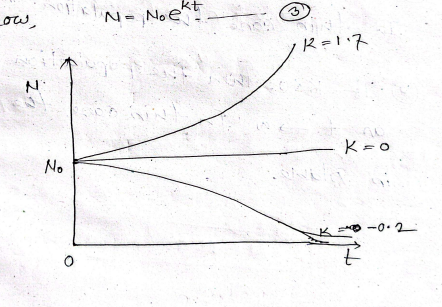
\includegraphics[]{Image/malthusian.png}
\end{center}
\section{Assume that, the population of Rajshahi city increases at a rate proportional to the number of inhabitants at any time $t$. If the population in double in 40 years, how many years it will be triple.}
According to the problem, we get:
\begin{align*}
    \frac{dN}{dt} &= kN \sidenote{1}
\end{align*}

The general solution of (1) is:
\begin{align*}
    N(t) &= N_0 e^{kt} \sidenote{2}
\end{align*}

Given that when $t = 40$, $N = 2N_0$:
\begin{align*}
    2N_0 &= N_0 e^{40k} \\
    40k &= \ln 2 \\
    k &= \frac{\ln 2}{40} \\
    \implies k &\approx 0.017328
\end{align*}

Suppose the population will triple in time $T$, i.e., $N(T) = 3N_0$:
\begin{align*}
    3N_0 &= N_0 e^{kT} \\
    e^{kT} &= 3 \\
    kT &= \ln 3 \\
    T &= \frac{\ln 3}{k} \\
    T &= \frac{\ln 3}{0.017328} \\
    \implies T &\approx 63.400986 \text{ years}
\end{align*}

So, the population will triple in $63.400986$ years (or approximately $63.40$ years from $t = 0$).
\section{Describe logistic model/Verhulst model. Find its solution. Also find the ultimate/maximum population.}
We have the Malthusian model:
\begin{align*}
    \frac{dN}{dt} &= kN \tag{1}
\end{align*}

The solution of (1) is:
\begin{align*}
    N &= N_0 e^{kt} \tag{2}
\end{align*}

We see that this solution gives accurate results only for small time and population. Therefore, we need to modify model (1). Verhulst assumed that $k$ is a function of population $N$ instead of a constant:
\begin{align*}
    \frac{dN}{dt} &= f(N) N \tag{3}
\end{align*}

From reality, when the population is small, it grows rapidly, and after a fixed amount of population, it decreases, i.e.:
\begin{align*}
    f(N) &= r - aN
\end{align*}

Therefore, equation (3) becomes:
\begin{align*}
    \frac{dN}{dt} &= (r - aN) N \\
    \implies \frac{dN}{dt} &= r \left(1 - \frac{aN}{r}\right) N \\
    \implies \frac{dN}{dt} &= r \left(1 - \frac{N}{K}\right) N \tag{4}
\end{align*}

where $K = \frac{r}{a}$ is the carrying capacity. Here, equation (4) is called the Verhulst or logistic population model.

---

\textbf{2nd Part: Solution of the Logistic Equation}

From (4), separating variables:
\begin{align*}
    \frac{dN}{N\left(1 - \frac{N}{K}\right)} &= r \, dt \\
    \left(\frac{1}{N} + \frac{\frac{1}{K}}{1 - \frac{N}{K}}\right) dN &= r \, dt
\end{align*}

Integrating both sides:
\begin{align*}
    \ln N + \frac{1}{K} \cdot \left(-K \ln\left(1 - \frac{N}{K}\right)\right) &= rt + \ln A \\
    \ln N - \ln\left(1 - \frac{N}{K}\right) &= rt + \ln A \\
    \ln\left(\frac{N}{1 - \frac{N}{K}}\right) &= rt + \ln A \\
    \frac{N}{1 - \frac{N}{K}} &= Ae^{rt} \\
    \frac{KN}{K - N} &= Ae^{rt}  \\
    \frac{KN}{K - N} &= A e^{rt} \tag{5}\\
    KN &= A(K - N) e^{rt} \\
    KN &= A K e^{rt} - A N e^{rt} \\
    N\left(K + A e^{rt}\right) &= A K e^{rt} \\
    N &= \frac{A K e^{rt}}{K + A e^{rt}} \tag{6}
\end{align*}

which is the general solution.

Suppose when $t = 0$, $N = N_0$. Then from equation (5):
\begin{align*}
    \frac{K N_0}{K - N_0} &= A e^{r(0)} \implies A = \frac{K N_0}{K - N_0}
\end{align*}

Substituting $A$ into equation (6):
\begin{align*}
    N &= \frac{K \left(\frac{K N_0}{K - N_0}\right) e^{rt}}{K + \left(\frac{K N_0}{K - N_0}\right) e^{rt}} \\
    &= \frac{K N_0 e^{rt}}{(K - N_0) + N_0 e^{rt}}
\end{align*}

Dividing numerator and denominator by $e^{rt}$:
\begin{align*}
    N &= \frac{K N_0}{N_0 + (K - N_0) e^{-rt}}
\end{align*}

which is the required particular solution.

---

\textbf{3rd Part: Ultimate Solution (Limiting Behavior)}

The maximum population (ultimate carrying capacity) as $t \to \infty$ is:
\begin{align*}
    N_{\max} &= \lim_{t \to \infty} \frac{K N_0}{N_0 + (K - N_0) e^{-rt}} \\
    &= \frac{K N_0}{N_0 + (K - N_0)(0)} \\
    &= \frac{K N_0}{N_0} = K \\
    \implies N_{\max} &= K
\end{align*}
\section{Find the equilibrium population of logistic model and discuss the stability.}
\textbf{Solution:}

We have the logistic model:
\begin{align*}
    \frac{dN}{dt} &= (r - aN)N \\
    &= r \left(1 - \frac{a}{r}N\right) N \\
    &= rN \left(1 - \frac{N}{K}\right) \tag{i}
\end{align*}

For equilibrium population,
\begin{align*}
    \frac{dN}{dt} &= 0\\
    rN \left(1 - \frac{N}{K}\right) &= 0\\
\text{or, } rN &= 0 \quad \text{or} \quad 1 - \frac{N}{K} = 0\\
\implies N &= 0 \quad \text{or} \quad N = K \quad (\because r \neq 0)
\end{align*}
which are the equilibrium populations.\\
\textbf{Case i: For $N = 0$}

Put $N = 0 + \varepsilon$, where $\varepsilon \ll 1$.Therefore, the model becomes:
\begin{align*}
    \frac{d(0 + \varepsilon)}{dt} &= r(0 + \varepsilon) \left(1 - \frac{0 + \varepsilon}{K}\right) \\
    \implies \frac{d\varepsilon}{dt} &= r\varepsilon \left(1 - \frac{\varepsilon}{K}\right) \\
    &= r\varepsilon \quad [\text{Neglecting } \varepsilon^2] \tag{ii}
\end{align*}
The solution of (ii) is:
   $ \varepsilon= \varepsilon_0 e^{rt}$
which is an unstable solution.
$$\therefore N = 0 \text{ is unstable.}$$
\textbf{Case ii: For $N = K$}

Put $N = K + \varepsilon$, where $\varepsilon \ll 1$.

Therefore, the model becomes:
\begin{align*}
    \frac{d(K + \varepsilon)}{dt} &= r(K + \varepsilon) \left(1 - \frac{K + \varepsilon}{K}\right) \\
    \implies \frac{dK}{dt} + \frac{d\varepsilon}{dt} &= r(K + \varepsilon) \left(1 - 1 - \frac{\varepsilon}{K}\right) \\
    \implies 0 + \frac{d\varepsilon}{dt} &= -\frac{r\varepsilon}{K} (K + \varepsilon) \\
    \implies \frac{d\varepsilon}{dt} &= -r\varepsilon \quad [\text{Neglecting } \varepsilon^2] \tag{iii}
\end{align*}

The solution of (iii) is:$\varepsilon = \varepsilon_0 e^{-rt}$
which decays to $0$ as $t \to \infty$.
$\therefore N = K \text{ is stable.}$
\section{Find the doubling time population for logistic model.}
We have:
\begin{align*}
    \frac{dN}{dt} &= r \left(1 - \frac{N}{K}\right) N \sidenote{1}
\end{align*}

We know the solution of (1) is:
\begin{align*}
    N &= \frac{N_0 K}{N_0 + (K - N_0) e^{-rt}} \sidenote{2}
\end{align*}

Suppose when $t$ becomes $T$, the population will double ($N = 2N_0$). Then from (2), we get:
\begin{align*}
    2N_0 &= \frac{N_0 K}{N_0 + (K - N_0) e^{-rT}} \\
    2N_0 \left[ N_0 + (K - N_0) e^{-rT} \right] &= N_0 K \\
    2N_0 + 2(K - N_0) e^{-rT} &= K \\
    2(K - N_0) e^{-rT} &= K - 2N_0 \\
    e^{-rT} &= \frac{K - 2N_0}{2(K - N_0)} \\
    e^{rT} &= \frac{2(K - N_0)}{K - 2N_0} \\
    rT &= \ln \left[ \frac{2(K - N_0)}{K - 2N_0} \right] \\
    \implies T &= \frac{1}{r} \ln \left[ \frac{2(K - N_0)}{K - 2N_0} \right] \sidenote{Required doubling time}
\end{align*}

which is the required doubling time.
\section{A population grows according to the model,
$$\frac{dN}{dt} = 1 - \exp\left[ 1 - r_0\left(1 - \frac{N}{K}\right) \right],$$
where $r_0$ and $K$ are positive constants. Determine the equilibrium state and its stability.}
\textbf{Solution:}

We have:
\begin{align*}
    \frac{dN}{dt} &= 1 - \exp\left[ 1 - r_0 \left(1 - \frac{N}{K}\right) \right] \sidenote{1}
\end{align*}

For equilibrium population, set $\frac{dN}{dt} = 0$:
\begin{align*}
    1 - \exp\left[ 1 - r_0 \left(1 - \frac{N}{K}\right) \right] &= 0 \\
    \exp\left[ 1 - r_0 \left(1 - \frac{N}{K}\right) \right] &= 1
\end{align*}

Taking natural logarithm on both sides:
\begin{align*}
    1 - r_0 \left(1 - \frac{N}{K}\right) &= 0 \\
    r_0 \left(1 - \frac{N}{K}\right) &= 1 \\
    1 - \frac{N}{K} &= \frac{1}{r_0} \\
    \frac{N}{K} &= 1 - \frac{1}{r_0} \\
    \implies N &= K \left(1 - \frac{1}{r_0}\right) \sidenote{Equilibrium population}
\end{align*}

which is the equilibrium population.\\
\textbf{Stability Analysis:}

Put $N = K \left(1 - \frac{1}{r_0}\right) + \varepsilon$, where $\varepsilon \ll 1$.

Substituting into (1):
\begin{align*}
    \frac{d}{dt} \left[ K \left(1 - \frac{1}{r_0}\right) + \varepsilon \right] &= 1 - \exp\left[ 1 - r_0 \left(1 - \frac{1}{K}\left[ K\left(1 - \frac{1}{r_0}\right) + \varepsilon \right]\right) \right] \\
    \frac{d\varepsilon}{dt} &= 1 - \exp\left[ 1 - r_0 \left(1 - 1 + \frac{1}{r_0} - \frac{\varepsilon}{K}\right) \right] \\
    &= 1 - \exp\left( \frac{\varepsilon r_0}{K} \right)
\end{align*}

Expanding using Taylor series:
\begin{align*}
    \frac{d\varepsilon}{dt} &= 1 - \left[ 1 + \frac{\varepsilon r_0}{K} + \frac{(\varepsilon r_0 / K)^2}{2!} + \dots \right] \\
    \frac{d\varepsilon}{dt} &= -\frac{\varepsilon r_0}{K} \sidenote{Neglecting higher-order terms of $\varepsilon$} \\
    \frac{d\varepsilon}{\varepsilon} &= -\frac{r_0}{K} \, dt \sidenote{2}
\end{align*}

Integrating (2):
\begin{align*}
    \varepsilon(t) &= \varepsilon_0 e^{-\frac{r_0}{K}t}
\end{align*}

As $t \to \infty$, $\varepsilon(t) \to 0$.

$$\therefore N^* = K \left(1 - \frac{1}{r_0}\right) \text{ is asymptotically stable.}$$
\section{The population $N$ of Rajshahi satisfy the Logistic model,
$$\frac{dN}{dt} = 0.03 N - 3 \times 10^{-8} N^2,$$
where $t$ is measured in years. If the population of Rajshahi was $2,00,000$ in 1980. What will be the population in the year 2000. What would be the possible maximum $\text{pop}^n$ of Rajshahi.}
\textbf{Solution:}

We have:
\begin{align*}
    \frac{dN}{dt} &= 0.03 N - 3 \times 10^{-8} N^2 \sidenote{1} \\
    &= 3 \times 10^{-2} N - 3 \times 10^{-8} N^2 \\
    &= 3 \times 10^{-2} N \left(1 - 10^{-6} N\right) \\
    \implies \frac{dN}{N \left(1 - 10^{-6} N\right)} &= 3 \times 10^{-2} \, dt \\
    \implies \left( \frac{1}{N} + \frac{10^{-6}}{1 - 10^{-6} N} \right) dN &= 3 \times 10^{-2} \, dt
\end{align*}

Integrating both sides:
\begin{align*}
    \ln N - \ln \left(1 - 10^{-6} N\right) &= 3 \times 10^{-2} t + \ln C \\
    \implies \ln \left( \frac{N}{1 - 10^{-6} N} \right) &= \ln \left( C e^{3 \times 10^{-2} t} \right) \\
    \implies \frac{N}{1 - 10^{-6} N} &= C e^{3 \times 10^{-2} t} \sidenote{A}
\end{align*}

When $t = 1980$, $N = 200000$:
\begin{align*}
    C &= \frac{200000 \, e^{-3 \times 10^{-2} \times 1980}}{1 - 10^{-6} \times 200000} \\
    &= \frac{200000 \, e^{-59.4}}{0.8} \\
    &= \frac{10^6}{4 e^{59.4}} \sidenote{decimal form}
\end{align*}

Substituting $C$ into equation (A):
\begin{align*}
    \frac{N}{1 - 10^{-6} N} &= \frac{10^6}{4 e^{59.4}} \cdot e^{3 \times 10^{-2} t} \\
    \frac{N}{1 - 10^{-6} N} &= \frac{10^6}{4 e^{59.4 - 0.03 t}} \\
    4 e^{59.4 - 0.03 t} N &= 10^6 \left(1 - 10^{-6} N\right) \\
    4 e^{59.4 - 0.03 t} N &= 10^6 - N \\
    N \left(1 + 4 e^{59.4 - 0.03 t}\right) &= 10^6 \\
    \implies N(t) &= \frac{10^6}{1 + 4 e^{59.4 - 0.03 t}} \sidenote{III}
\end{align*}

which is the particular solution.

---

\textbf{Calculations:}

Substituting $t = 2000$ into (III):
\begin{align*}
    N &= \frac{10^6}{1 + 4 e^{59.4 - 0.03 \times 2000}} \\
    &= \frac{10^6}{1 + 4 e^{-0.6}} \\
    &= 312964.89 \approx 312965 \sidenote{Required population}
\end{align*}

Maximum population limit:
\begin{align*}
    N_{\max} &= \lim_{t \to \infty} \frac{10^6}{1 + 4 e^{59.4 - 0.03 t}} \\
    &= 10^6
\end{align*}
\section{If the carrying capacity of the logistic model is $K$ and $0 < N_0 < \frac{K}{2}$, then determine the time of doubling of population.\textcolor{green}{2018}}
\textbf{Solution:}

We have the solution of the logistic model:
\begin{align*}
    N &= \frac{K N_0}{N_0 + (K - N_0) e^{-rt}} \sidenote{i}
\end{align*}

Suppose when $t = T$, the population $N_0$ will double, i.e., $N = 2N_0$.

Putting this in (i), we get:
\begin{align*}
    2N_0 &= \frac{K N_0}{N_0 + (K - N_0) e^{-rT}} \\
    2 \left[ N_0 + (K - N_0) e^{-rT} \right] &= K \\
    (K - N_0) e^{-rT} &= \frac{K}{2} - N_0 \\
    (K - N_0) e^{-rT} &= \frac{K - 2N_0}{2} \\
    e^{-rT} &= \frac{K - 2N_0}{2(K - N_0)} \\
    e^{rT} &= \frac{2(K - N_0)}{K - 2N_0} \\
    rT &= \ln \left[ \frac{2(K - N_0)}{K - 2N_0} \right] \\
    T &= \frac{1}{r} \ln \left[ \frac{2(K - N_0)}{2\left(\frac{K}{2} - N_0\right)} \right] \\
    T &= \frac{1}{r} \ln \left[ \frac{K - N_0}{\frac{K}{2} - N_0} \right]
\end{align*}

Since $0 < N_0 < \frac{K}{2}$, the fraction $\frac{K - N_0}{\frac{K}{2} - N_0}$ is positive (and greater than $1$).

$$\therefore \text{The doubling time is } T = \frac{1}{r} \ln \left[ \frac{K - N_0}{\frac{K}{2} - N_0} \right]$$
\section{The world's population was estimated to be $5000$ million in $1950$ and $7500$ million in $2000$. Estimate the population of the world in the year $2050$, given that the population increases according to the Malthusian model.\textcolor{green}{2023}}
The Malthusian model of population growth is governed by the differential equation:
\begin{equation}
    \frac{dN}{dt} = kN \tag{i}
\end{equation}

where:
\begin{itemize}
    \item $N(t)$ is the population (in millions) at time $t$ (in years).
    \item $k$ is the relative growth rate parameter.
\end{itemize}

Separating variables in equation (i):
\begin{equation*}
    \frac{dN}{N} = k \, dt
\end{equation*}

Integrating both sides:
\begin{align*}
    \int \frac{dN}{N} &= \int k \, dt \\[1ex]
    \ln N &= kt + \ln N_0 \\[1ex]
    \ln\left(\frac{N}{N_0}\right) &= kt \\[1ex]
    \implies N(t) &= N_0 e^{kt} \tag{ii}
\end{align*}

---

Let $t = 0$ correspond to the year 1950.
\begin{itemize}
    \item At $t = 0$ (1950): $N(0) = N_0 = 5000 \text{ million}$
    \item At $t = 50$ (2000): $N(50) = 7500 \text{ million}$
    \item At $t = 100$ (2050): $N(100) = \,?$
\end{itemize}

From equation (ii), when $t = 50$:
\begin{align*}
    N(50) &= N_0 e^{50k} \\[1ex]
    7500 &= 5000 e^{50k} \\[1ex]
    \implies e^{50k} &= \frac{7500}{5000} \\[1ex]
    \implies e^{50k} &= 1.5 \tag{iii}
\end{align*}
For the year 2050, the elapsed time from 1950 is $t = 100$ years:
\begin{align*}
    N(100) &= N_0 e^{100k} \\[1ex]
    N(100) &= 5000 e^{100k}
\end{align*}

Using the laws of exponents:
\begin{equation*}
    N(100) = 5000 \left(e^{50k}\right)^2
\end{equation*}

Substituting equation (iii) into this expression:
\begin{align*}
    N(100) &= 5000 \times (1.5)^2 \\[1ex]
    N(100) &= 5000 \times 2.25 \\[1ex]
    N(100) &= 11250 \text{ million}
\end{align*}

\textbf{Ans:} The estimated population of the world in the year 2050 is \textbf{11,250 million} (or \textbf{11.25 billion}).
\section{Suppose the population of Bangladesh grows according to the Malthusian model. The population of Bangladesh was estimated to be $170.00\text{ million}$ in $2010$ and $180.00\text{ million}$ in $2020$. Estimate the population of Bangladesh in the year $2030$ and also in $2040$.\textcolor{green}{2021}}
\textbf{Solution:}

The Malthusian model is given by:
\begin{equation}
    \frac{dN}{dt} = kN \tag{i}
\end{equation}

The solution to this model is:
\begin{equation}
    N = N_0 e^{k(t - t_0)} \tag{ii}
\end{equation}

---

\textbf{1st Case:}

Here,
\begin{align*}
    N &= 180.00 \text{ million} \\
    N_0 &= 170.00 \text{ million} \\
    t_0 &= 2010 \\
    t &= 2020
\end{align*}

From equation (ii):
\begin{align*}
    180 &= 170 \, e^{k(2020 - 2010)} \\
    \implies e^{10k} &= \frac{180}{170} = \frac{18}{17} \\
    \implies k &= \frac{1}{10} \ln\left(\frac{18}{17}\right) \\
    &= 0.0057158
\end{align*}

Substituting $k$ back into equation (ii):
\begin{equation}
    N = N_0 e^{0.0057158(t - t_0)} \tag{iii}
\end{equation}

---

\textbf{2nd Case:}

Here,
\begin{align*}
    N_0 &= 180.00 \text{ million} \\
    t_0 &= 2020 \\
    t &= 2030
\end{align*}

From equation (iii), we get:
\begin{align*}
    N &= 180 \, e^{0.0057158 \times (2030 - 2020)} \\
    &= 180 \, e^{0.0057158 \times 10} \\
    &= 190 \text{ million}
\end{align*}

---

\textbf{3rd Case:}

Here,
\begin{align*}
    N_0 &= 190 \text{ million} \\
    t_0 &= 2030 \\
    t &= 2040
\end{align*}

Calculating the updated growth rate parameter $k$:
\begin{align*}
    k &= \frac{1}{10} \ln\left(\frac{19}{18}\right) \\
    &= 5.40672 \times 10^{-3} \\
    &= 0.00540672
\end{align*}

Estimating population for the year 2040:
\begin{align*}
    N &= 190 \, e^{0.00540672 \times (2040 - 2030)} \\
    &= 200.555 \text{ million} \quad \mathbf{(\text{Ans})}
\end{align*}
\section{If $\frac{dP}{dt} = rP - k$, $P(0) = P_0$, then solve this equation and make a realistic comment regarding the solution.\textcolor{green}{2020}}
\textbf{Solution:}

Given differential equation:
\begin{equation*}
    \frac{dP}{dt} = rP - k, \quad P(0) = P_0
\end{equation*}

Separating variables:
\begin{align*}
    \frac{dP}{rP - k} &= dt \\[1ex]
    \frac{dP}{r\left(P - \frac{k}{r}\right)} &= dt \\[1ex]
    \implies \frac{dP}{P - \frac{k}{r}} &= r \, dt
\end{align*}

Integrating both sides:
\begin{align*}
    \int \frac{dP}{P - \frac{k}{r}} &= \int r \, dt \\[1ex]
    \ln\left(P - \frac{k}{r}\right) &= rt + c \\[1ex]
    P - \frac{k}{r} &= e^{rt + c} \\[1ex]
    P - \frac{k}{r} &= A e^{rt} \quad \text{where } A = e^c \\[1ex]
    \implies P &= \frac{k}{r} + A e^{rt} \tag{i}
\end{align*}

Applying the initial condition $P(0) = P_0$:
\begin{align*}
    P_0 &= \frac{k}{r} + A e^0 \\[1ex]
    \implies A &= P_0 - \frac{k}{r}
\end{align*}

Substituting $A$ into equation (i):
\begin{equation}
    P(t) = \frac{k}{r} + \left(P_0 - \frac{k}{r}\right)e^{rt} \tag{ii}
\end{equation}

which is the required solution.\\

From equation (ii), the dynamics of the population depend on the initial population $P_0$ relative to the critical threshold $\frac{k}{r}$:

\begin{itemize}
    \item \textbf{Growth Phase $\left(P_0 > \frac{k}{r}\right)$:} 
    If the initial population $P_0$ is greater than $\frac{k}{r}$, the term $\left(P_0 - \frac{k}{r}\right)$ is positive, causing $P(t)$ to grow exponentially over time.

    \item \textbf{Extinction Phase $\left(P_0 < \frac{k}{r}\right)$:} 
    If the initial population $P_0$ is less than $\frac{k}{r}$, the harvesting rate $k$ exceeds the natural growth rate $rP_0$. Consequently, $P(t)$ decreases over time and eventually reaches zero (extinction).

    \item \textbf{Equilibrium Phase $\left(P_0 = \frac{k}{r}\right)$:} 
    If $P_0 = \frac{k}{r}$, the population remains perfectly constant at $P(t) = \frac{k}{r}$ for all time $t \ge 0$.
\end{itemize}
\chapter{Discrete population Model}
\section*{Something Important}
\begin{itemize}
    \item Malthusian Population Model:
    $$\frac{dN}{dt} = k N$$
    $N(t)$ = population size at time $t$, $k$ = constant growth rate parameter ($k = b - d$, where $b$ is the per-capita birth rate and $d$ is the per-capita death rate)\\
    solution: $N(t) = N_0 e^{kt}$
    \item Logistic (Verhulst) Population Model
    $$\frac{dN}{dt} = r N \left(1 - \frac{N}{K}\right)$$Its explicit solution is:$$N(t) = \frac{K N_0}{N_0 + (K - N_0) e^{-rt}}$$
    $r$ is the intrinsic growth rate and $k$ is carrying capacity
    \item Harvesting model:
    $$\frac{dN}{dt} = rN \left(1 - \frac{N}{K}\right) \pm EN $$
    Solution:
    $$N(t) = \frac{(r \pm E) N_0}{\frac{r}{K} N_0 + \left( (r \pm E) - \frac{r}{K} N_0 \right) e^{-(r \pm E)t}}$$

    

\end{itemize}
\section{Describe the Harvesting Population Model and find its solutions. Discuss the stability of the Harvesting Model.}
\section*{Solution of Harvesting / Migration Model}

We have the standard logistic model:
\begin{equation}
\frac{dN}{dt} = rN \left(1 - \frac{N}{K}\right) \tag{i}
\end{equation}

The mortality rate may be affected by the migration of population from one place to another. The migration is due to better jobs, better weather, better housing, or oppression by the government, etc.

The migration rate is also proportional to the number of population. The logistic model becomes:
\begin{equation}
\frac{dN}{dt} = rN \left(1 - \frac{N}{K}\right) \pm EN \tag{ii}
\end{equation}
where $E$ is the proportionality constant in the harvesting/migration model, and $r, K, E$ are positive constants. $r$ is called the per capita growth rate, and $K$ is the carrying capacity of the environment.

\subsection*{Solution of the Differential Equation}

From ii we have:
\begin{align*}
\frac{dN}{dt} &= rN \pm EN - \frac{rN^2}{K} \\
&= N(r \pm E) - \frac{r}{K}N^2 \\
\frac{dN}{dt} &= aN - bN^2 \tag{A}
\end{align*}
where $a = r \pm E$ and $b = \dfrac{r}{K}$.

Separating variables:
\begin{align*}
\frac{dN}{N(a - bN)} &= dt\\
\Rightarrow \left( \frac{1}{N} + \frac{b}{a - bN} \right) dN &= a \, dt
\end{align*}

Integrating both sides:
\begin{align*}
\ln N - \ln(a - bN) &= at + \ln c \\
\ln \left( \frac{N}{a - bN} \right) &= \ln \left( c e^{at} \right) \\
\frac{N}{a - bN} &= c e^{at} \\
N &= (a - bN) c e^{at} \tag{iii}
\end{align*}

Applying the initial condition $N(0) = N_0$ at $t = 0$:
\begin{equation*}
N_0 = (a - bN_0)c \implies c = \frac{N_0}{a - bN_0}
\end{equation*}

Substituting $c$ back into iii:
\begin{align*}
N &= \left( \frac{a - bN}{a - bN_0} \right) N_0 e^{at} \\
N + b \frac{N N_0 e^{at}}{a - bN_0} &= \frac{a N_0 e^{at}}{a - bN_0} \\
N \left( 1 + \frac{b N_0 e^{at}}{a - bN_0} \right) &= \frac{a N_0 e^{at}}{a - bN_0} \\
N \left( \frac{a - bN_0 + b N_0 e^{at}}{a - bN_0} \right) &= \frac{a N_0 e^{at}}{a - bN_0} \\
N &= \frac{a N_0 e^{at}}{(a - bN_0) + b N_0 e^{at}}
\end{align*}

Dividing numerator and denominator by $e^{at}$:
\begin{equation*}
N(t) = \frac{a N_0}{b N_0 + (a - bN_0)e^{-at}}
\end{equation*}

Substituting back $a = r \pm E$ and $b = \dfrac{r}{K}$:
\begin{equation*}
N(t) = \frac{(r \pm E) N_0}{\frac{r}{K} N_0 + \left( (r \pm E) - \frac{r}{K} N_0 \right) e^{-(r \pm E)t}}
\end{equation*}
which gives the required population solution.

\subsection*{Stability Analysis}

For equilibrium states, set $\dfrac{dN}{dt} = 0$.

From equation A:
\begin{align*}
aN - bN^2 &= 0 \\
N(a - bN) &= 0 \\
\implies N = 0 \quad &\text{or} \quad N = \frac{a}{b}
\end{align*}

\paragraph{Case 1: Stability near $N = 0$}
Let $N = 0 + \varepsilon$, where $\varepsilon$ is a small perturbation.
\begin{align*}
\frac{d\varepsilon}{dt} &= r\varepsilon \left(1 - \frac{\varepsilon}{K}\right) \pm E\varepsilon \\
&\approx r\varepsilon \pm E\varepsilon \quad (\text{neglecting } \varepsilon^2) \\
\frac{d\varepsilon}{dt} &= (r \pm E)\varepsilon = a\varepsilon
\end{align*}

This is a Malthusian model with solution:
\begin{equation*}
\varepsilon(t) = \varepsilon_0 e^{at}
\end{equation*}
For $a > 0$, $\varepsilon(t)$ grows exponentially, so $N = 0$ is an **unstable** equilibrium solution.

\paragraph{Case 2: Solution at Equilibrium $N = \frac{a}{b}$}
Here $N = \frac{a}{b} = \frac{K}{r}(r \pm E)$.

\begin{enumerate}
    \item **When $E = 0$ (No harvesting/migration):**
    \begin{equation*}
    N(t) = \frac{r N_0}{\frac{r}{K} N_0 + \left( r - \frac{r}{K} N_0 \right) e^{-rt}}
    \end{equation*}
    which is the standard solution of the logistic population model. The equilibrium population $N = K$ is **stable**.

    \item **If $E > r$ (Over-harvesting):**
    The growth rate becomes negative ($a < 0$). The population will continuously decrease and eventually vanish ($N \to 0$).

    \item **If $E < r$ (Sustainable harvesting):**
    $a > 0$, so the population stays positive, increases toward the modified carrying capacity, and exists sustainably.
\end{enumerate}
\section{Determine the extinction time and tripling time  population govern by the Model }
$$ \frac{dN}{dt} = N(4-N) - 4$$
\section*{Population Extinction and Tripling Time}

Given that,
\begin{align*}
    \frac{dN}{dt} &= N(4-N) - 4 \\
    \Rightarrow \frac{dN}{dt} &= 4N - N^2 - 4 \\
    \Rightarrow \frac{dN}{dt} &= -(N-2)^2 \\
    \Rightarrow \frac{dN}{(N-2)^2} &= -dt \sidenote{separating variables} \\
    \Rightarrow -(N-2)^{-1} &= -t - c \sidenote{by integrating} \\
    \Rightarrow \frac{1}{N-2} &= t + c
\end{align*}

When $t = 0$, $N = N_0$,
\begin{align*}
    \Rightarrow c &= \frac{1}{N_0 - 2}
\end{align*}

\begin{align*}
    \therefore \frac{1}{N-2} &= t + \frac{1}{N_0 - 2} \\
    \Rightarrow \frac{1}{N-2} &= \frac{(N_0 - 2)t + 1}{N_0 - 2} \\
    \Rightarrow N - 2 &= \frac{N_0 - 2}{(N_0 - 2)t + 1} \sidenote{taking reciprocal} \\
    \Rightarrow N &= \frac{2(N_0 - 2)t + 2 + N_0 - 2}{(N_0 - 2)t + 1} \\
    \Rightarrow N &= \frac{2(N_0 - 2)t + N_0}{(N_0 - 2)t + 1} \\
    \Rightarrow N &= \frac{N_0 + 2N_0 t - 4t}{(N_0 - 2)t + 1}
\end{align*}

Suppose $t = T$, $N = 0$,
\begin{align*}
    N_0 + 2N_0 T - 4T &= 0 \\
    \Rightarrow 4T - 2T N_0 &= N_0 \\
    \Rightarrow T &= \frac{N_0}{4 - 2N_0} \\
    \Rightarrow T &= \frac{N_0}{2(2 - N_0)}, \quad 0 < N_0 < 2
\end{align*}
which is required time.

\vspace{1em}
\noindent\textbf{Note: Tripling time,} \\
Suppose when $t \to T$, the population $N$ will be $3N_0$, then
\begin{align*}
    3N_0 &= \frac{N_0(2T + 1) - 4T}{N_0 T - 2T + 1} \\
    \Rightarrow 3N_0^2 T - 6N_0 T + 3N_0 &= 2N_0 T + N_0 - 4T \sidenote{by cross-multiplying} \\
    \Rightarrow 3N_0^2 T - 8N_0 T + 2N_0 + 4T &= 0 \\
    \Rightarrow 3N_0^2 T - 8N_0 T + 4T &= -2N_0 \\
    \Rightarrow T(3N_0^2 - 8N_0 + 4) &= -2N_0 \\
    \therefore T &= \frac{-2N_0}{3N_0^2 - 8N_0 + 4}
\end{align*}
\section{ Describe the two species linear competition model and identify it.\textcolor{red}{(not CL)}}
Let $x$ and $y$ be two competitor species. Then the model is:

\begin{align*}
    \frac{dx}{dt} &= ax - by \sidenote{i} \\
    \frac{dy}{dt} &= -cx + dy \quad ; \, a,b,c,d > 0 \sidenote{ii}
\end{align*}

This is called the \textbf{linear competition model}.\\
\textbf{Identification:}

From equation (i), we observe that in the absence of $y$ ($y = 0$), $x$ increases ($\frac{dx}{dt} = ax > 0$), and in the presence of $y$, the growth rate of $x$ decreases due to the $-by$ term.

Again, from equation (ii), we observe that in the absence of $x$ ($x = 0$), the $y$ population increases ($\frac{dy}{dt} = dy > 0$), and in the presence of $x$, the $y$ population decreases due to the $-cx$ term.

$$\therefore \text{Therefore, this is a } \mathbf{two\text{-}species \ linear \ competition \ model.}$$
\section{Describe the symbiotic population model and explain it.\textcolor{red}{(not CL)}}
\textbf{Solution:}

Let $x$ and $y$ be two populations. Then the model is:

\begin{align*}
    \left.
    \begin{aligned}
        \frac{dx}{dt} &= -ax + by \\[1ex]
        \frac{dy}{dt} &= cx - dy
    \end{aligned}
    \right\} \sidenote{i}
\end{align*}
This is called the \textbf{linear symbiotic model}\\
Here, $a, b, c, d > 0$.


\textbf{Explanation:}

From the 1st equation of (i), we observe that in the absence of $y$ ($y = 0$), $x$ decreases ($\frac{dx}{dt} = -ax < 0$), and in the presence of $y$, the $x$ population increases due to the $+by$ term.

From the 2nd equation of (i), we observe that in the absence of $x$ ($x = 0$), $y$ decreases ($\frac{dy}{dt} = -dy < 0$), and in the presence of $x$, the growth rate of $y$ increases due to the $+cx$ term.

$$\therefore \text{Therefore, this is a } \mathbf{two\text{-}species \ symbiotic \ model.}$$
\section{The population $N(t)$ (in million) of Bangladesh satisfies the model $\frac{dN}{dt} = \alpha N - \beta N^2$ where $t$ is measured in years. If $N(2000) = 127.66$, $N(2010) = 147.56$ and $N(2020) = 164.67$, find the population of Bangladesh in 2030.\textcolor{green}{(2020)}}
\textbf{Solution:}

Given model:
\begin{align*}
    \frac{dN}{dt} &= \alpha N - \beta N^2  \\
    \implies \frac{dN}{N(\alpha - \beta N)} &= dt \\
    \implies \frac{1}{\alpha} \left( \frac{1}{N} + \frac{\beta}{\alpha - \beta N} \right) dN &= dt \\
    \implies \ln N - \ln(\alpha - \beta N) &= \alpha t + \ln C \\
    \implies \ln \left( \frac{N}{\alpha - \beta N} \right) &= \ln \left( C e^{\alpha t} \right) \\
    \implies \frac{N}{\alpha - \beta N} &= C e^{\alpha t}
\end{align*}

Let $A = C$:
\begin{align*}
    \frac{N}{\alpha - \beta N} &= A e^{\alpha t} 
\end{align*}

\textbf{Solving for $N(t)$:}

\begin{align*}
    N &= A e^{\alpha t} (\alpha - \beta N) \\
    N + \beta A e^{\alpha t} N &= A \alpha e^{\alpha t} \\
    N \left(1 + \beta A e^{\alpha t}\right) &= A \alpha e^{\alpha t} \\
    N &= \frac{A \alpha e^{\alpha t}}{1 + \beta A e^{\alpha t}} = \frac{\alpha}{\beta + \frac{1}{A} e^{-\alpha t}}
\end{align*}

Let $c = \frac{1}{A}$:
\begin{align*}
    N(t) &= \frac{\alpha}{\beta + c e^{-\alpha t}} \sidenote{i}
\end{align*}

which is the required solution at any time $t$.

---

\textbf{Given initial/boundary conditions:}
\begin{itemize}
    \item $N(2000) = 127.66$
    \item $N(2010) = 147.56$
    \item $N(2020) = 164.67$
\end{itemize}

From the solution formula:
\begin{align*}
    N(2000) &= \frac{\alpha}{\beta + c e^{-2000\alpha}} \\
    \implies 127.66 &= \frac{\alpha}{\beta + c e^{-2000\alpha}} \sidenote{ii} \\[1ex]
    147.56 &= \frac{\alpha}{\beta + c e^{-2010\alpha}} \sidenote{iii} \\[1ex]
    164.67 &= \frac{\alpha}{\beta + c e^{-2020\alpha}} \sidenote{iv}
\end{align*}

Dividing (ii) by (iii):
\begin{align*}
    \frac{127.66}{147.56} &= \frac{\beta + c e^{-2010\alpha}}{\beta + c e^{-2000\alpha}} \\
    \frac{127.66}{147.56} - 1 &= \frac{\beta + c e^{-2010\alpha}}{\beta + c e^{-2000\alpha}} - 1 \\
    \frac{127.66 - 147.56}{147.56} &= \frac{c \left(e^{-2010\alpha} - e^{-2000\alpha}\right)}{\beta + c e^{-2000\alpha}} \\
    \frac{-19.90}{147.56} &= \frac{c \left(e^{-2010\alpha} - e^{-2000\alpha}\right)}{\beta + c e^{-2000\alpha}} \sidenote{v}
\end{align*}

Dividing equation (ii) by (iv):
\begin{align*}
    \frac{127.66}{164.67} &= \frac{\beta + c e^{-2020\alpha}}{\beta + c e^{-2000\alpha}} \\
    \implies \frac{127.66 - 164.67}{164.67} &= \frac{c \left(e^{-2020\alpha} - e^{-2000\alpha}\right)}{\beta + c e^{-2000\alpha}} \\
    \implies \frac{-37.01}{164.67} &= \frac{c \left(e^{-2020\alpha} - e^{-2000\alpha}\right)}{\beta + c e^{-2000\alpha}} \sidenote{vii}
\end{align*}
Dividing (v) by (vii):
\begin{align*}
    \left(\frac{-19.90}{147.56}\right) \times \left(\frac{164.67}{-37.01}\right) &= \frac{e^{-2010\alpha} - e^{-2000\alpha}}{e^{-2020\alpha} - e^{-2000\alpha}} \\
    \implies 0.600039 &= \frac{e^{-2000\alpha}\left(e^{-10\alpha} - 1\right)}{e^{-2000\alpha}\left(e^{-20\alpha} - 1\right)} \\
    \implies 0.600039 &= \frac{e^{-10\alpha} - 1}{e^{-20\alpha} - 1} = \frac{e^{-10\alpha} - 1}{\left(e^{-10\alpha}\right)^2 - 1} \\
    \implies 0.600039 &= \frac{1}{e^{-10\alpha} + 1} \\
    \implies e^{-10\alpha} + 1 &= 1.666558 \\
    \implies e^{-10\alpha} &= 0.666558 \\
    \implies \alpha &= -\frac{1}{10} \ln(0.666558) \\
    \implies \alpha &= 0.0405628
\end{align*}

---

From equations (iii) and (iv):
\begin{align*}
    \beta + c e^{-2010\alpha} &= \frac{\alpha}{147.56 \times 10^6} \sidenote{viii} \\[1ex]
    \beta + c e^{-2020\alpha} &= \frac{\alpha}{164.67 \times 10^6} \sidenote{ix}
\end{align*}

Subtracting (ix) - (viii):
\begin{align*}
    c\left(e^{-2020\alpha} - e^{-2010\alpha}\right) &= \frac{\alpha}{10^6} \left(\frac{1}{164.67} - \frac{1}{147.56}\right) \\
    \implies c &= \frac{0.0405628}{10^6 \times \left(e^{-2020\alpha} - e^{-2010\alpha}\right)} \left(\frac{1}{164.67} - \frac{1}{147.56}\right) \\
    \implies c &= 2.19455 \times 10^{25}
\end{align*}

From equation (viii):
\begin{align*}
    \beta + 2.19455 \times 10^{25} \times e^{-2010 \times 0.0405628} &= \frac{0.0405628}{147.56 \times 10^6} \\
    \implies \beta + 8.56609 \times 10^{-11} &= 2.74890 \times 10^{-10} \\
    \implies \beta &= 2.74890 \times 10^{-10} - 8.56609 \times 10^{-11} \\
    \implies \beta &= 1.892283 \times 10^{-10}
\end{align*}

When $t = 2030$:
\begin{align*}
    N(2030) &= \frac{0.0405628}{1.892283 \times 10^{-10} + 2.19455 \times 10^{25} e^{-0.0405628 \times 2030}} \\
    &= \frac{0.0405628}{2.272884 \times 10^{-10}} \\
    &\approx 178463981.7
\end{align*}

$$\mathbf{N(2030) \approx 178.46 \text{ million}}$$
\chapter{Two species Population Model}
\section*{Important Info:}
\begin{itemize}
    \item linear predator prey model
   \begin{align*}
    \frac{dx}{dt} &= -ax + by \sidenote{1} \\
    \frac{dy}{dt} &= dy - cx \;; \quad a, b, c, d > 0 \sidenote{2}
\end{align*}
\end{itemize}
\section{Describe the two species linear predator prey model and explain it.}
\textbf{Solution:} Let $x$ denote the predator population and $y$ denote the prey population.

\noindent Then the model:
\begin{align*}
    \frac{dx}{dt} &= -ax + by \sidenote{1} \\
    \frac{dy}{dt} &= dy - cx \;; \quad a, b, c, d > 0 \sidenote{2}
\end{align*}
is called the two-species linear predator-prey model.

\vspace{1em}
\noindent\textbf{2nd part / (Explanation):}

\noindent From equation (1), we observe that in the absence of prey ($y = 0$), $\frac{dx}{dt} = -ax$, meaning the predator population $x$ decays exponentially. When prey is present ($by > 0$), it contributes positively to predator growth.

\vspace{0.5em}
\noindent From equation (2), we observe that in the absence of predators ($x = 0$), $\frac{dy}{dt} = dy$, meaning the prey population $y$ grows exponentially (Malthusian growth). When predators are present ($-cx < 0$), predation reduces prey population growth.

\begin{align*}
    \therefore \text{The model is a two-species linear predator-prey model.}
\end{align*}
\section{Identify and solve the two species linear population model.}
\textbf{Solution:} Given that
\begin{align*}
    \frac{dx}{dt} &= -x + 4y \sidenote{i} \\
    \frac{dy}{dt} &= 5y - 2x \sidenote{ii}
\end{align*}

\noindent From equation (i), we observe that in absence of $y$, the $x$ population decreases and in presence of $y$, the $x$ population increases.

\vspace{0.5em}
\noindent Again, from equation (ii), we observe that in absence of $x$, the $y$ population increases and in presence of $x$, the $y$ population decreases.

\begin{align*}
    \therefore \text{The model is a predator--prey population model.}
\end{align*}

\vspace{1em}
\noindent\textbf{2nd part:} The model can be written as
\begin{align*}
    (D + 1)x - 4y &= 0 \sidenote{iii} \\
    2x + (D - 5)y &= 0 \sidenote{iv}
\end{align*}
where $D = \frac{d}{dt}$.

\vspace{0.5em}
\noindent Now, multiplying (iii) by $(D - 5)$ and (iv) by $4$ and adding:
\begin{align*}
    (D + 1)(D - 5)x - 4(D - 5)y &= 0 \\
    8x + 4(D - 5)y &= 0 \\
    \hline
    (D + 1)(D - 5)x + 8x &= 0 \\
    \Rightarrow (D^2 - 4D - 5)x + 8x &= 0 \\
    \Rightarrow (D^2 - 4D - 5 + 8)x &= 0 \\
    \Rightarrow (D^2 - 4D + 3)x &= 0 \sidenote{v}
\end{align*}

The trial solution of (v) is $x = ce^{mt}$.

\begin{align*}
    \therefore \text{The Auxiliary equation } m^2 - 4m + 3 &= 0 \\
    \Rightarrow (m - 3)(m - 1) &= 0 \\
    \Rightarrow m &= 1, 3
\end{align*}

\begin{align*}
    \therefore \text{The general solution is } x &= c_1 e^t + c_2 e^{3t} \sidenote{vi}
\end{align*}

\noindent Putting the value in (iii):
\begin{align*}
    (D + 1)(c_1 e^t + c_2 e^{3t}) &= 4y \\
    \Rightarrow 4y &= D(c_1 e^t + c_2 e^{3t}) + c_1 e^t + c_2 e^{3t} \\
    \Rightarrow 4y &= c_1 e^t + 3c_2 e^{3t} + c_1 e^t + c_2 e^{3t} \\
    \Rightarrow y &= \frac{1}{2} c_1 e^t + c_2 e^{3t} \sidenote{Answer}
\end{align*}
\section{State and explain the Latka-Volterra predator prey model}
\section*{Also find the exact solution and make a stability analysis and sketch the phase portrait of the population dynamics}
\subsection*{ Statement and Explanation of the Model}

Let $x(t)$ denote the prey population density and $y(t)$ denote the predator population density at time $t$. The classic Lotka--Volterra system is defined by:

\begin{align*}
    \frac{dx}{dt} &= \alpha x - \beta xy \sidenote{1} \\
    \frac{dy}{dt} &= -\gamma y + \delta xy \sidenote{2}
\end{align*}
where parameters $\alpha, \beta, \gamma, \delta > 0$.

\vspace{0.5em}
\begin{itemize}
    \item $\alpha x$: Exponential growth of prey in the absence of predators.
    \item $-\beta xy$: Rate of prey mortality due to predation (proportional to interaction frequency).
    \item $-\gamma y$: Exponential death/decay rate of predators in the absence of prey.
    \item $\delta xy$: Rate of predator population increase resulting from consuming prey.
\end{itemize}

\vspace{1em}
\noindent\textbf{Explanation:}

\noindent From the prey equation, we observe that in the absence of predators, the prey population increases without limit, and in the presence of predators, the growth rate of the prey population is reduced by an amount proportional to the predator population present.

\vspace{0.5em}
\noindent Similarly, from the predator equation, we find that in the absence of prey, the predator population decreases and becomes extinct due to starvation; and in the presence of the prey population, the growth rate of the predator population is increased by an amount proportional to the prey population present.
\subsection*{Exact Solution}

\noindent The model (1) can be written as:
\begin{align*}
    \frac{dy}{dx} &= \frac{y(-\gamma + \delta x)}{x(\alpha - \beta y)} \\
    \Rightarrow \frac{dy}{dx} &= \frac{xy\left(-\frac{\gamma}{x} + \delta\right)}{xy\left(\frac{\alpha}{y} - \beta\right)} \\
    \Rightarrow \frac{dy}{dx} &= \frac{\delta - \frac{\gamma}{x}}{\frac{\alpha}{y} - \beta} \\
    \Rightarrow \left(\frac{\alpha}{y} - \beta\right) dy &= \left(\delta - \frac{\gamma}{x}\right) dx \sidenote{separating variables} \\
    \Rightarrow \alpha \frac{dy}{y} - \beta \, dy &= \delta \, dx - \gamma \frac{dx}{x}
\end{align*}

\noindent Integrating, we get:
\begin{align*}
    \alpha \ln y - \beta y &= \delta x - \gamma \ln x + \ln k \sidenote{by integrating} \\
    \Rightarrow \ln y^\alpha - \ln e^{\beta y} &= \ln e^{\delta x} - \ln x^\gamma + \ln k \\
    \Rightarrow \ln y^\alpha - \ln e^{\beta y} - \ln e^{\delta x} + \ln x^\gamma &= \ln k \\
    \Rightarrow \ln \frac{y^\alpha}{e^{\beta y}} + \ln \frac{x^\gamma}{e^{\delta x}} &= \ln k \\
    \Rightarrow \ln \frac{x^\gamma y^\alpha}{e^{\delta x} e^{\beta y}} &= \ln k \\
    \Rightarrow \frac{x^\gamma y^\alpha}{e^{\delta x + \beta y}} &= k \sidenote{II}
\end{align*}

where $k$ is the integral constant, which is the \textbf{general solution}.

\vspace{1em}
\noindent Using initial conditions $x(0) = x_0$ and $y(0) = y_0$, we get:
\begin{align*}
    \frac{x_0^\gamma y_0^\alpha}{e^{\delta x_0} e^{\beta y_0}} &= k
\end{align*}

\noindent Putting the value of $k$ in (II), we get:
\begin{align*}
    \frac{x^\gamma y^\alpha}{e^{\delta x} e^{\beta y}} &= \frac{x_0^\gamma y_0^\alpha}{e^{\delta x_0} e^{\beta y_0}} \sidenote{III}
\end{align*}
which is the \textbf{particular solution} of (1).

\vspace{1em}
\noindent Using $f(x) = \frac{x^\gamma}{e^{\delta x}}$ and $g(y) = \frac{y^\alpha}{e^{\beta y}}$:
\begin{align*}
    \therefore f(x) \cdot g(y) &= K \sidenote{IV}
\end{align*}
\subsection*{ Extrema Analysis for $f(x)$}

From (IV), it is observed that $f(x)$ and $g(y)$ are inversely related.

\vspace{0.5em}
\noindent Also, $f(0) = 0$ when $x = 0$, and $f(x) \to 0$ as $x \to \infty$.

\vspace{1em}
\noindent Now,
\begin{align*}
    \frac{df}{dx} &= (\gamma - \delta x) x^{\gamma - 1} e^{-\delta x}
\end{align*}

\noindent and
\begin{align*}
    \frac{d^2 f}{dx^2} &= \left[(\gamma - \delta x)^2 - \gamma \right] x^{\gamma - 2} e^{-\delta x}
\end{align*}

\noindent For optimum value, $\frac{df}{dx} = 0$:
\begin{align*}
    \therefore (\gamma - \delta x) x^{\gamma - 1} e^{-\delta x} = 0 \implies x = \frac{\gamma}{\delta}
\end{align*}

\noindent Now for $x = \frac{\gamma}{\delta}$:
\begin{align*}
    \frac{d^2 f}{dx^2} &= \left[(\gamma - \gamma)^2 - \gamma\right] \left(\frac{\gamma}{\delta}\right)^{\gamma - 2} e^{-\gamma} = -\gamma \left(\frac{\gamma}{\delta}\right)^{\gamma - 2} e^{-\gamma} \\
    \therefore \frac{d^2 f}{dx^2} &< 0
\end{align*}

\vspace{0.5em}
\noindent Hence, $f(x)$ has a \textbf{local maximum} at $x = \frac{\gamma}{\delta}$.\\
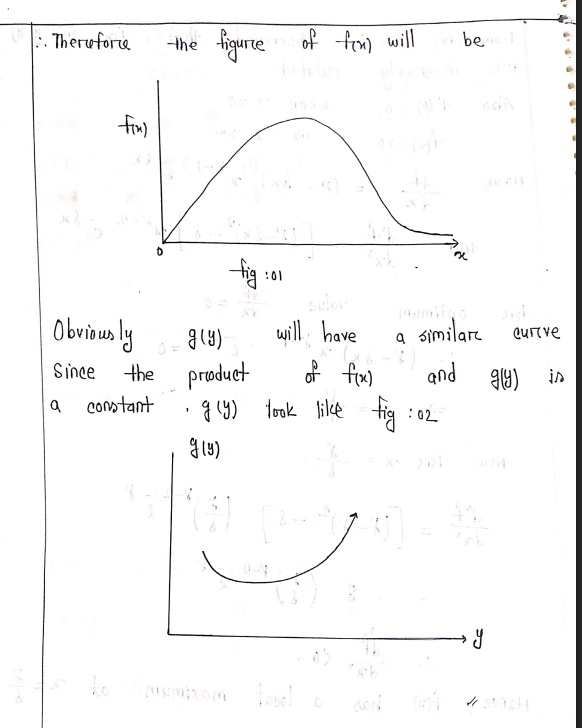
\includegraphics[]{Image/Lotka volterra1.png}
\subsection*{Stability Analysis}

System (i) cannot be solved to find $x(t)$ and $y(t)$ explicitly, so the exact path of (i) cannot be drawn. We look for points where the population remains constant (for an indefinite time) and find the paths of (i) in the neighborhood of these equilibrium points.

\vspace{0.5em}
\noindent The equilibrium points of (i) are given by:
\begin{align*}
    \left.
    \begin{aligned}
        x(\alpha - \beta y) &= 0 \\
        y(-\gamma + \delta x) &= 0
    \end{aligned}
    \right\} \sidenote{v}
\end{align*}

\noindent Solving (v), we find the equilibrium points $A(0, 0)$ and $B\left(\frac{\gamma}{\delta}, \frac{\alpha}{\beta}\right)$.

\vspace{0.5em}
\noindent We note that these are also solutions of (i) which are independent of time and can be considered as special cases in which the curves degenerate into points.

\vspace{0.5em}
\noindent We now investigate the stability of $A(0, 0)$ and $B\left(\frac{\gamma}{\delta}, \frac{\alpha}{\beta}\right)$.

\vspace{1em}
\noindent\textbf{Case I --- Equilibrium Point $A(0, 0)$:}

\noindent This is the case where both the prey and the predator populations are absent. Thus, when the populations are sufficiently close to this point, we can neglect the second terms $\beta xy$ and $\delta xy$ of (i) in comparison to the first terms. Hence, (i) reduces to:
\begin{align*}
    \left.
    \begin{aligned}
        \frac{dx}{dt} &= \alpha x \\
        \frac{dy}{dt} &= -\gamma y
    \end{aligned}
    \right\} \sidenote{vi}
\end{align*}

\noindent with solutions:
\begin{align*}
    x(t) = c_1 e^{\alpha t} \quad \text{and} \quad y(t) = c_2 e^{-\gamma t} \sidenote{vii}
\end{align*}

where $c_1$ and $c_2$ are arbitrary constants. Since $x$ and $y$ are non-negative, we must have $c_1 \ge 0$, $c_2 \ge 0$, and the family of curves described by (vii) is shown in \textbf{fig: 03}.

\vspace{0.5em}
\noindent Further, if we displace the population slightly from the equilibrium point $(0, 0)$, then it tends to move away from the point $(0, 0)$.
\begin{align*}
    \therefore \text{The equilibrium point } A(0, 0) \text{ is } \textbf{unstable}.
\end{align*}
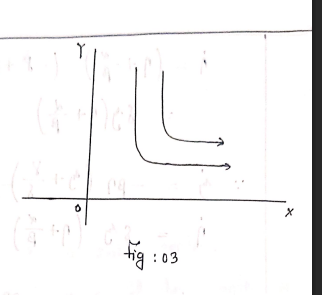
\includegraphics[]{Image/Lotka-volterra3.png}
\subsection*{Case II --- Equilibrium Point $B\left(\frac{\gamma}{\delta}, \frac{\alpha}{\beta}\right)$ Perturbation}

\vspace{0.5em}
\noindent This is the case where both species are present. We consider (i) by using:
\begin{align*}
    \left.
    \begin{aligned}
        x &= \xi + \frac{\gamma}{\delta} \\
        y &= \eta + \frac{\alpha}{\beta}
    \end{aligned}
    \right\} \sidenote{ix}
\end{align*}
\begin{align*}
    \frac{d\xi}{dt} &= \left(\xi + \frac{\gamma}{\delta}\right) (\alpha - \beta\eta - \alpha) = -\beta\eta \left(\xi + \frac{\gamma}{\delta}\right) \\
    \therefore \dot{\xi} &= -\beta\eta \left(\xi + \frac{\gamma}{\delta}\right) \\
    \implies \dot{\xi} &= -\beta\xi\eta - \frac{\gamma\beta}{\delta}\eta \\
   \therefore \text{Similarly}\, \dot{\eta} &= \delta\xi\eta + \frac{\alpha\delta}{\beta}\xi
\end{align*}

\noindent Since $\xi$ and $\eta$ are small, we can neglect the non-linear terms of $\xi\eta$:
\begin{align*}
    \left.
    \begin{aligned}
        \dot{\xi} &= -\frac{\gamma\beta}{\delta} \eta =a\xi + b\eta \\
        \dot{\eta} &= \frac{\alpha\delta}{\beta} \xi=c\xi + d\eta
    \end{aligned}
    \right\} \sidenote{x}
\end{align*}

\noindent Here $a = 0, b = -\frac{\gamma\beta}{\delta}, c = \frac{\alpha\delta}{\beta}, d = 0$.(linearized equation)

\vspace{0.5em}
\noindent $\therefore$ The characteristic equation is:
\begin{align*}
    \lambda^2 - (a + d)\lambda + (ad - bc) = 0
\end{align*}
\begin{align*}
    \implies \lambda^2 - (0 + 0) + \left(0 + \frac{\gamma\beta}{\delta} \cdot \frac{\alpha\delta}{\beta}\right) &= 0 \\
    \implies \lambda^2 &= -\alpha\gamma \\
    \implies \lambda &= \pm \sqrt{-\alpha\gamma} \\
    \therefore \lambda &= \pm i\sqrt{\alpha\gamma}
\end{align*}

\noindent Thus, $B\left(\frac{\gamma}{\delta}, \frac{\alpha}{\beta}\right)$ is a \textbf{stable center}(Eigen value is purely imaginary).
\noindent To know the exact shape of the center, we eliminate $t$ from (x) and obtain:
\begin{align*}
    \frac{d\xi}{d\eta} &= \frac{-\frac{\gamma\beta}{\delta}\eta}{\frac{\alpha\delta}{\beta}\xi} = -\frac{\gamma\beta}{\delta}\eta \times \frac{\beta}{\alpha\delta\xi} = -\frac{\gamma\beta^2}{\alpha\delta^2} \frac{\eta}{\xi} \\
    \implies \xi \, d\xi &= -\frac{\gamma\beta^2}{\alpha\delta^2} \eta \, d\eta \\
    \implies \frac{1}{\gamma\beta^2} \xi \, d\xi + \frac{1}{\alpha\delta^2} \eta \, d\eta &= 0
\end{align*}

\noindent Integrating, we get:
\begin{align*}
    \frac{1}{\gamma\beta^2} \frac{\xi^2}{2} + \frac{1}{\alpha\delta^2} \frac{\eta^2}{2} &= \frac{c^2}{2} \\
    \implies \frac{\xi^2}{\gamma\beta^2} + \frac{\eta^2}{\alpha\delta^2} &= c^2 \\
    \implies \frac{\xi^2}{\gamma\beta^2 c^2} + \frac{\eta^2}{\alpha\delta^2 c^2} &= 1 \sidenote{xi}
\end{align*}

where $c$ is a constant.

\vspace{0.5em}
\noindent This represents a family of \textbf{concentric ellipses}. We find from (xi) that the directions of the ellipses are \textbf{anti-clockwise}.(eqn x has different sign) Hence, the stable center $B\left(\frac{\gamma}{\delta}, \frac{\alpha}{\beta}\right)$ is shown in \textbf{fig: 04}.
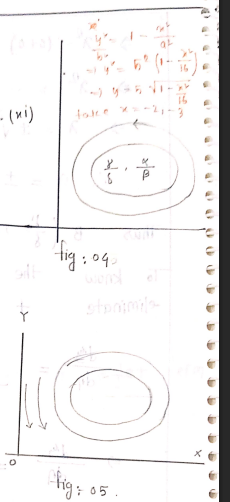
\includegraphics[]{Image/Lotka4.png}

\vspace{0.5em}
\noindent From \textbf{fig: 01}, it is clear that for any value of $f(x)$, there are either two values of $x$ or none. Same arguments hold for $y$ also. This implies that the path of (i) is a \textbf{closed loop} as shown in \textbf{fig: 05}.

\vspace{0.5em}
\noindent Hence, from \textbf{fig: 03}, \textbf{fig: 04}, and \textbf{fig: 05}, the population dynamics of (i) near its equilibrium points are shown in the phase plane.
\section{Problem: Two-Species Competition Model\textcolor{green}{2021}}

Identify and solve the two-species linear population model:
\begin{align*}
    \frac{dx}{dt} &= 3x - y \sidenote{$x(0) = 95$} \\
    \frac{dy}{dt} &= -2x + 2y \sidenote{$y(0) = 165$}
\end{align*}
Determine the time when the population will become extinct.

\bigskip
\noindent \textbf{1st Part: Model Identification}

Consider the system of differential equations:
\begin{align*}
    \frac{dx}{dt} &= 3x - y \tag{1a} \\
    \frac{dy}{dt} &= -2x + 2y \tag{1b}
\end{align*}

From equation (1a), in the absence of $y$, $x$ increases, whereas in the presence of $y$, $x$ decreases. From equation (1b), in the absence of $x$, $y$ increases, whereas in the presence of $x$, $y$ decreases. 

Since both species inhibit each other's growth rate, system (1) is a \textbf{competition model}.

\bigskip
\noindent \textbf{2nd Part: General Solution}

Using the differential operator $D = \frac{d}{dt}$:
\begin{align*}
    (D - 3)x + y &= 0 \tag{ii} \\
    2x + (D - 2)y &= 0 \tag{iii}
\end{align*}

Applying $[(\text{ii}) \times (D - 2) - (\text{iii})]$:
\begin{align*}
    (D - 3)(D - 2)x + (D - 2)y - 2x - (D - 2)y &= 0 \\
    (D^2 - 5D + 6)x - 2x &= 0 \sidenote{eliminating $y$} \\
    (D^2 - 5D + 4)x &= 0 \tag{iv}
\end{align*}

Equation (iv) is a homogeneous linear 2nd-order differential equation. Let $x = e^{mt}$ be a trial solution:
\begin{align*}
    m^2 - 5m + 4 &= 0 \sidenote{since $e^{mt} \neq 0$} \\
    (m - 1)(m - 4) &= 0 \implies m = 1, 4
\end{align*}

Hence, the general solution for $x(t)$ is:
\begin{align*}
    x(t) = c_1 e^t + c_2 e^{4t}
\end{align*}

Expressing $y(t)$ using equation (1a):
\begin{align*}
    y &= 3x - \frac{dx}{dt} \sidenote{from (1a)} \\
    y &= 3(c_1 e^t + c_2 e^{4t}) - \frac{d}{dt}(c_1 e^t + c_2 e^{4t}) \\
    y &= 3c_1 e^t + 3c_2 e^{4t} - (c_1 e^t + 4c_2 e^{4t}) \\
    \implies y(t) &= 2c_1 e^t - c_2 e^{4t}
\end{align*}

Thus, the general solution of the model is:
\begin{align*}
    x(t) &= c_1 e^t + c_2 e^{4t} \tag{v} \\
    y(t) &= 2c_1 e^t - c_2 e^{4t}
\end{align*}

\bigskip
\noindent \textbf{3rd Part: Particular Solution \& Extinction Analysis}

Applying initial conditions $x(0) = 95$ and $y(0) = 165$:
\begin{align*}
    95 &= c_1 + c_2 \\
    165 &= 2c_1 - c_2
\end{align*}

Adding both equations gives $3c_1 = 260 \implies c_1 = \frac{260}{3}$, which yields $c_2 = 95 - \frac{260}{3} = \frac{25}{3}$. The particular solution is:
\begin{align*}
    x(t) &= \frac{260}{3} e^t + \frac{25}{3} e^{4t} \tag{vi} \\
    y(t) &= \frac{520}{3} e^t - \frac{25}{3} e^{4t} \tag{vii}
\end{align*}

\bigskip
\noindent \textbf{Extinction Time Determination:}

Let $t = T$ be the extinction time where population reaches zero.

\noindent \textbf{For species $x$:}
\begin{align*}
    0 &= \frac{260}{3} e^T + \frac{25}{3} e^{4T} \sidenote{set $x(T) = 0$} \\
    e^{3T} &= -\frac{260}{25} \implies T = \frac{1}{3} \ln\left(-\frac{260}{25}\right)
\end{align*}
Since $\ln(-260/25) \notin \mathbb{R}$, population $x$ will \textbf{never become extinct}.

\smallskip
\noindent \textbf{For species $y$:}
\begin{align*}
    0 &= \frac{520}{3} e^T - \frac{25}{3} e^{4T} \sidenote{set $y(T) = 0$} \\
    e^{3T} &= \frac{520}{25} = \frac{104}{5} \\
    \implies T &= \frac{1}{3} \ln\left(\frac{104}{5}\right) \approx 1.0118
\end{align*}
Since $T > 0$ is real and positive, species $y$ will become \textbf{extinct at time $T = \frac{1}{3} \ln\left(\frac{104}{5}\right)$}.
\section{ Identify and solve the two-species linear population model:}
\begin{align*}
    \frac{dx}{dt} &= -2x + 4y \sidenote{$x(0) = 100$} \\
    \frac{dy}{dt} &= x - 2y   \sidenote{$y(0) = 300$}
\end{align*}
\section*{Also find the time when the population will become extinct.\textcolor{green}{2020}}
\noindent \textbf{Solution:}

\noindent \textbf{1st Part: Model Identification}

Given system of differential equations:
\begin{align*}
    \frac{dx}{dt} &= -2x + 4y \tag{i} \\
    \frac{dy}{dt} &= x - 2y   \tag{ii}
\end{align*}

From equation (i), in the absence of $y$, the growth rate of $x$ decreases, while in the presence of $y$, the growth rate of $x$ increases. Similarly, from equation (ii), in the absence of $x$, the growth rate of $y$ decreases, while in the presence of $x$, the growth rate of $y$ increases.

Therefore, the system represents a \textbf{symbiotic model}.

\bigskip
\noindent \textbf{2nd Part: General Solution}

Using the differential operator $D = \frac{d}{dt}$:
\begin{align*}
    (D + 2)x - 4y &= 0 \tag{iii}\\
    -x + (D + 2)y &= 0 \tag{iv}
\end{align*}

Operating $(D + 2)$ on (iii) and multiplying (iv) by $4$:
\begin{align*}
    (D + 2)^2 x - 4(D + 2)y &= 0 \\
    -4x + 4(D + 2)y &= 0
\end{align*}

Adding both equations eliminates $y$:
\begin{align*}
    \left[(D + 2)^2 - 4\right]x &= 0 \sidenote{eliminating $y$} \\
    (D^2 + 4D)x &= 0 \\
    \implies \frac{d^2x}{dt^2} + 4\frac{dx}{dt} &= 0 \tag{v}
\end{align*}

Let $x = e^{mt}$ be a trial solution of (v). The auxiliary equation is:
\begin{align*}
    m^2 + 4m &= 0 \\
    m(m + 4) &= 0 \implies m = 0, -4
\end{align*}

Hence, the general solution for $x(t)$ is:
\begin{align*}
    x(t) = c_1 + c_2 e^{-4t} \tag{vi}
\end{align*}

Substituting equation (vi) into equation (i) to solve for $y(t)$:
\begin{align*}
    4y &= \frac{dx}{dt} + 2x \sidenote{from (i)} \\
    4y &= -4c_2 e^{-4t} + 2(c_1 + c_2 e^{-4t}) \\
    4y &= 2c_1 - 2c_2 e^{-4t} \\
    \implies y(t) &= \frac{1}{2}c_1 - \frac{1}{2}c_2 e^{-4t} \tag{vii}
\end{align*}

Equations (vi) and (vii) are the general solution.\\
\noindent \textbf{3rd Part: Particular Solution}

Applying initial conditions $x(0) = 100$ and $y(0) = 300$:
\begin{align*}
    100 &= c_1 + c_2 \tag{viii} \\
    300 &= \frac{1}{2}c_1 - \frac{1}{2}c_2 \tag{ix}
\end{align*}

From equation (viii), $c_1 = 100 - c_2$. Substituting into (ix):
\begin{align*}
    300 &= \frac{1}{2}(100 - c_2) - \frac{1}{2}c_2 \\
    300 &= 50 - c_2 \implies c_2 = -250 \\
    \implies c_1 &= 100 - (-250) = 350
\end{align*}

Substituting $c_1$ and $c_2$ gives the particular solution:
\begin{align*}
    x(t) &= 350 - 250 e^{-4t} \tag{x} \\
    y(t) &= 175 + 125 e^{-4t} \tag{xi}
\end{align*}

\bigskip
\noindent \textbf{4th Part: Extinction Time Analysis}

Let $t = T$ be the extinction time where population reaches $0$.

\noindent \textbf{For species $x$:}
\begin{align*}
    0 &= 350 - 250 e^{-4T} \tag{xii}\\
    250 e^{-4T} &= 350 \\
    e^{-4T} &= \frac{35}{25} = \frac{7}{5} \\
    \ln(e^{-4T}) &= \ln\left(\frac{7}{5}\right) \\
    -4T &= \ln\left(\frac{7}{5}\right) \implies T = -\frac{1}{4}\ln\left(\frac{7}{5}\right)
\end{align*}
Since time cannot be negative ($T < 0$), the $x$ population will \textbf{never go extinct}.

\smallskip
\noindent \textbf{For species $y$:}
\begin{align*}
    0 &= 175 + 125 e^{-4T} \tag{xiii} \\
    e^{-4T} &= -\frac{175}{125} = -\frac{7}{5} \\
    -4T &= \ln\left(-\frac{7}{5}\right) \implies T = -\frac{1}{4}\ln\left(-\frac{7}{5}\right)
\end{align*}
Since $\ln(-7/5)$ is undefined in the real numbers ($\mathbb{R}$), the $y$ population will \textbf{never go extinct}.\\
\textit{Check page 146, 2 math}
\chapter{Epidemic/Infection disease Model}
\section*{Info:}
\begin{itemize}
    \item SIR Model:
    \begin{align}
    \frac{dS}{dt} &= -\beta S I \tag{1} \\
    \frac{dI}{dt} &= \beta S I - \gamma I \tag{2} \\
    \frac{dR}{dt} &= \gamma I \tag{3}
\end{align}
\end{itemize}
\section{Describe the simple SIR epidemic model. Find the condition on which the infection will ultimately die out or spread throughout the population.}
\subsection*{Description of the Simple SIR Epidemic Model}

The \textbf{SIR model} (Kermack and McKendrick, 1927) divides a fixed total population $N$ into three compartmental classes:

\begin{itemize}
    \item $S(t)$: \textbf{Susceptible} individuals who are healthy but vulnerable to catching the disease.
    \item $I(t)$: \textbf{Infected} individuals who currently have the disease and can transmit it to susceptibles.
    \item $R(t)$: \textbf{Removed} (or Recovered) individuals who have either recovered with permanent immunity or died.
\end{itemize}
\noindent\textbf{Model Assumptions:}
\begin{enumerate}
    \item The total population $N$ remains constant over the epidemic time scale (i.e., no births, natural deaths, or migration):
    \[
        S(t) + I(t) + R(t) = N = \text{constant}
    \]
    \item Infection rate is proportional to the rate of contact between susceptible and infected individuals ($\beta S I$).
    \item Recovery rate is directly proportional to the number of infected individuals ($\gamma I$).
\end{enumerate}
\noindent\textbf{Differential Equations:}
\begin{align}
    \frac{dS}{dt} &= -\beta S I \tag{1} \\
    \frac{dI}{dt} &= \beta S I - \gamma I \tag{2} \\
    \frac{dR}{dt} &= \gamma I \tag{3}
\end{align}
\noindent where:
\begin{itemize}
    \item $\beta > 0$ is the \textbf{transmission (infection) rate coefficient}.
    \item $\gamma > 0$ is the \textbf{recovery/removal rate coefficient}.
\end{itemize}
The initial conditions of the above model are:
\[
S(0) = S_0 > 0, \quad I(0) = I_0 > 0, \quad \text{and} \quad R(0) = 0
\]
\noindent Initially, from equation (2):
\begin{align*}
    \frac{dI}{dt} &= \beta S I - \alpha I \\
    \implies \frac{dI}{dt} &= I \beta \left(S - \frac{\alpha}{\beta}\right)
\end{align*}
\noindent Evaluating at $t = 0$:
\begin{align*}
    \left. \frac{dI}{dt} \right|_{t=0} &= I_0 \beta \left(S_0 - \frac{\alpha}{\beta}\right) \tag{iv}
\end{align*}
\noindent From $\frac{dS}{dt} = -\beta S I$, since $\beta, S, I$ are positive, we have $\frac{dS}{dt} < 0$, which implies $S(t)$ is a strictly decreasing function. Therefore:
\[
S(t) < S(0) = S_0 \quad \text{for all } t > 0
\]
\subsection*{Case 1: No Epidemic Outbreak $\left(S_0 \le \frac{\alpha}{\beta}\right)$}
\noindent From equation (iv):
\begin{align*}
    \frac{dI}{dt} = I \beta \left(S - \frac{\alpha}{\beta}\right) &< I \beta \left(S_0 - \frac{\alpha}{\beta}\right) \quad \text{since } S(t) < S_0
\end{align*}
\noindent Now, if $S_0 \le \frac{\alpha}{\beta}$:
\begin{align*}
    \frac{dI}{dt} &< \beta I \left(\frac{\alpha}{\beta} - \frac{\alpha}{\beta}\right) = 0 \\
    \implies \frac{dI}{dt} &< 0 \quad \text{for all } t \ge 0
\end{align*}

\noindent Thus, $I(t)$ is a strictly decreasing function. Integrating gives:
\begin{align*}
    [I]_0^t &< 0 \implies I(t) < I_0 \\
    \implies \lim_{t \to \infty} I(t) &< I_0
\end{align*}
Hence, no epidemic occurs, and the infection dies out.

\vspace{1em}
\subsection*{Case 2: Epidemic Outbreak $\left(S_0 > \frac{\alpha}{\beta}\right)$}

\noindent Let $S_0 > \frac{\alpha}{\beta}$. From equation (iv):
\begin{align*}
    \left. \frac{dI}{dt} \right|_{t=0} &= I_0 \beta \left(S_0 - \frac{\alpha}{\beta}\right) > 0 \\
    \implies \left. \frac{dI}{dt} \right|_{t=0} &> 0
\end{align*}

\noindent Since the derivative is positive at $t = 0$, $I(t)$ is initially an increasing function. Thus, for early times $t > 0$:
\[
I(t) > I(0) = I_0
\]

\noindent The number of infected individuals increases initially. Hence, an **epidemic occurs** and the infection spreads through the population.
\section{Discuss the deterministic susceptible infected(SI) model and solve. Show that the infection will spread throughout the population.}
\section*{Solution:}

The \textbf{SI model} is the simplest mathematical framework for describing the spread of an infectious disease in a closed population without recovery or immunity.

\subsection*{Assumptions:}
\begin{enumerate}
    \item The total population size $N$ is fixed and constant over time:
    \[
    S(t) + I(t) = N
    \]
    where:
    \begin{itemize}
        \item $S(t)$ is the number of \textbf{susceptible} individuals at time $t$.
        \item $I(t)$ is the number of \textbf{infected} individuals at time $t$.
    \end{itemize}
    \item The rate of new infections is proportional to the product of susceptible individuals $S(t)$ and infected individuals $I(t)$ (mass-action principle).
    \item Once an individual becomes infected, they remain infected indefinitely (no recovery or removal).
\end{enumerate}

\subsection*{Governing Differential Equations:}
\begin{align*}
    \frac{dS}{dt} &= -\beta S I  \\[0.8em]
    \frac{dI}{dt} &= \beta S I 
\end{align*}

\noindent where $\beta > 0$ is the transmission or infection rate parameter.
\noindent The total population size is given by:
\subsection*{Solving for $S(t)$}
Let \begin{equation}
    \text{total population} = S(t) + I(t) = n + 1 \sidenote{1}
\end{equation}
\noindent From Equation (2), we have:
\[
\frac{dS}{dt} = -\beta SI
\]
Substituting $I(t) = (n + 1) - S(t)$ from Equation (1):
\[
I(t) = (n + 1) - S(t)
\]
We get:
\begin{align*}
    \frac{dS}{dt} &= -\beta S \left( (n + 1) - S \right) \\
    \implies \frac{dS}{-S \left( (n + 1) - S \right)} &= \beta \, dt \\
    \implies -\frac{1}{n + 1} \left( \frac{1}{S} + \frac{1}{n + 1 - S} \right) dS &= \beta \, dt
\end{align*}

\noindent Integrating both sides:
\[
-\left\{ \ln S - \ln(n + 1 - S) \right\} = (n + 1)\beta t + \ln c
\]
\[
\implies \ln \left( \frac{n + 1 - S}{S} \right) = (n + 1)\beta t + \ln c
\]

\noindent Applying initial conditions ($t = 0, S = n$):
\[
\ln \left( \frac{1}{n} \right) = \ln c \implies c = \frac{1}{n}
\]

\noindent Substituting $c$ back into the integral equation:
\begin{align*}
    \ln \left( \frac{n + 1 - S}{S} \right) &= (n + 1)\beta t + \ln \left( \frac{1}{n} \right) \\
    \implies \ln \left( \frac{\frac{n + 1 - S}{S}}{\frac{1}{n}} \right) &= (n + 1)\beta t \\
    \implies \ln \left\{ \frac{n(n + 1 - S)}{S} \right\} &= (n + 1)\beta t \\
    \implies \frac{n(n + 1 - S)}{S} &= e^{(n + 1)\beta t} \\
    \implies n^2 + n - Sn &= S e^{(n + 1)\beta t} \\
    \implies S \left[ n + e^{(n + 1)\beta t} \right] &= n(n + 1) \\
    \implies S(t) &= \frac{n(n + 1)}{n + e^{(n + 1)\beta t}} \sidenote{5}
\end{align*}

\subsection*{Solving for $I(t)$}

\noindent Now, considering the differential equation for infected individuals:
\begin{align*}
    \frac{dI}{dt} &= \beta SI = \beta \left( (n + 1) - I \right) I \\
    \implies \frac{dI}{I(n + 1 - I)} &= \beta \, dt \\
    \implies \frac{1}{n + 1} \left( \frac{1}{I} + \frac{1}{n + 1 - I} \right) dI &= \beta \, dt \\
    \implies \ln I - \ln(n + 1 - I) &= (n + 1)\beta t + \ln c \\
    \implies \ln \left\{ \frac{I}{n + 1 - I} \right\} &= (n + 1)\beta t + \ln c
\end{align*}

\noindent At $t = 0, I = 1$:
\[
\ln \left\{ \frac{1}{n + 1 - 1} \right\} = \ln c \implies c = \frac{1}{n}
\]

\noindent Substituting $c$:
\begin{align*}
    \implies \frac{I}{n + 1 - I} &= \frac{1}{n} e^{(n + 1)\beta t} \\
    \implies I(t) &= \frac{n + 1}{1 + n e^{-(n + 1)\beta t}} \sidenote{6}
\end{align*}

\subsection*{3. Limiting Behavior as $t \to \infty$}

\noindent Taking limits as $t \to \infty$:
\[
\lim_{t \to \infty} S(t) = \lim_{t \to \infty} \frac{n(n + 1)}{n + e^{(n + 1)\beta t}} = 0
\]
\noindent From (6):
\[
\lim_{t \to \infty} I(t) = \lim_{t \to \infty} \frac{n + 1}{1 + n e^{-(n + 1)\beta t}} = n + 1
\]

\noindent So, the infection will spread throughout the entire population.
\chapter{HIV}
\section{Describe the deterministic AIDS model. Show that the infection spread throughout the population. Find the doubling time. Also find the number of AIDS patients at any time $t$.}
\noindent\textbf{Solution.}\ Let $N(t)$ denote the size of the total population. Let $S(t)$, $I(t)$, $A(t)$ and $H(t)$ denote, respectively, the number of susceptibles, infected population, AIDS patients, and the number of HIV-positive population who are non-infectious.

Now we consider the following flow chart:

\begin{center}
\begin{tikzpicture}[node distance=1.6cm and 2.2cm, >=stealth, thick]
    \node (B) {};
    \node[below=0.6cm of B] (S) {Susceptible $S(t)$};
    \node[below=1.4cm of S] (I) {Infectious $I(t)$};
    \node[below left=1.6cm and 1.4cm of I] (A) {AIDS $A(t)$};
    \node[below right=1.6cm and 0.6cm of I] (H) {Seropositive non-infectious $H(t)$};
    \node[right=1.8cm of S] (Sd) {Natural death};
    \node[right=1.8cm of I] (Id) {Natural death};
    \node[left=1.8cm of A] (Ad) {Natural death};
    \node[below=1cm of A] (Dd) {Disease induced death};
    \node[right=2.2cm of H] (Hd) {Natural death};

    \draw[->] (B) -- node[right]{$B$} (S);
    \draw[->] (S) -- node[right]{$\lambda c$} (I);
    \draw[->] (S) -- node[above]{$\mu$} (Sd);
    \draw[->] (I) -- node[above]{$\mu$} (Id);
    \draw[->] (I) -- node[above left]{$p\nu$} (A);
    \draw[->] (I) -- node[above right]{$(1-p)\nu$} (H);
    \draw[->] (A) -- node[above]{$\mu$} (Ad);
    \draw[->] (A) -- node[right]{$d$} (Dd);
    \draw[->] (H) -- node[above]{$\mu$} (Hd);
\end{tikzpicture}
\end{center}

Here $B$ is the recruitment of susceptibles, $\mu$ is the natural (non-AIDS) death rate, $\lambda c$ is the rate of transferral from susceptible to the infectious class, $\lambda$ is the probability of acquiring infection from a randomly chosen partner
\begin{align*}
    \left(\lambda = \frac{\beta I}{N}\right),
\end{align*}
where $\beta$ is the transmission probability, $c$ is the number of partners, $d$ is the AIDS-related death rate, $p$ is the proportion of HIV-positive who are infectious, and $\nu$ is the rate of conversion from infection to AIDS, here taken to be constant. $\dfrac{1}{\nu}$, say $=D$, is the average incubation time of the disease.

Therefore, a reasonable model based on the flow chart is
\begin{align*}
    \frac{dS}{dt} &= B - \mu S - \lambda c S, \qquad \lambda = \frac{\beta I}{N} \sidenote{1} \\
    \frac{dI}{dt} &= \lambda c S - (\nu+\mu)I \sidenote{2} \\
    \frac{dA}{dt} &= p\nu I - (d+\mu)A \sidenote{3} \\
    \frac{dH}{dt} &= (1-p)\nu I - \mu H \sidenote{4} \\
    N(t) &= S(t) + I(t) + H(t) + A(t) \sidenote{5}
\end{align*}

Now, differentiating (5) w.r.t.\ $t$, we get
\begin{align*}
    \frac{dN}{dt} &= \frac{dS}{dt} + \frac{dI}{dt} + \frac{dH}{dt} + \frac{dA}{dt} \\
    &= \big[B - \mu S - \lambda c S\big] + \big[\lambda c S - (\nu+\mu)I\big] + \big[(1-p)\nu I - \mu H\big] + \big[p\nu I - (d+\mu)A\big] \\
    &= B - \mu S - \mu I - \mu H - (d+\mu)A \\
    &= B - \mu(S+I+H+A) - dA \\
    \Rightarrow\ \frac{dN}{dt} &= B - \mu N - dA. \sidenote{6}
\end{align*}

Now, if at $t=0$ an infected individual is introduced into an otherwise infection-free population of susceptibles, then we have, near $t=0$, $N \approx S$. Therefore, from (2), we get
\begin{align*}
    \frac{dI}{dt} &\approx \lambda c N - (\nu+\mu)I, \qquad \text{since } N \approx S \\
    \frac{dI}{dt} &\approx c\left(\frac{\beta I}{N}\right)N - (\nu+\mu)I \\
    \Rightarrow\ \frac{dI}{dt} &\approx (\beta c - \nu - \mu)I \sidenote{7} \\
    \Rightarrow\ \frac{dI}{dt} &\approx \nu\left(\frac{\beta c}{\nu} - \frac{\mu}{\nu} - 1\right)I
\end{align*}

Since the average incubation time $\dfrac{1}{\nu}$ is very much shorter than the average life expectancy $\dfrac{1}{\mu}$, so $\dfrac{\mu}{\nu} \approx 0$. Therefore, from (7), we get
\begin{align*}
    \frac{dI}{dt} \approx \nu(R_0 - 1)I, \qquad \text{where } R_0 \approx \frac{\beta c}{\nu} > 1.
\end{align*}
Thus the basic reproductive rate $R_0$ is given in terms of the number of partners $c$, the transmission probability $\beta$, and the average incubation time of the disease $\dfrac{1}{\nu}$.

Now, we can get some interesting information from the analysis of the system (1)--(5) during the early stages of an epidemic. Here the population consists of almost all susceptibles, and so $N \approx S$. Therefore, the growth rate of infection, i.e.\ the HIV-positive $I$ class, is approximated by equation (8). The solution of (8) is
\begin{align*}
    I(t) = I(0)\,e^{\nu(R_0-1)t} = I(0)\,e^{rt}, \sidenote{10}
\end{align*}
where $r = \nu(R_0-1)$ is positive only if an epidemic exists (i.e.\ $R_0 > 1$), and $I(0)$ is the initial number of people introduced into the susceptible population.

From (10), we observe that $I(t)$, i.e.\ infection, grows exponentially, and ultimately the whole population will be infected.

\vspace{0.2cm}
\noindent\textbf{Doubling time.}\ Suppose the doubling time is $t_d$, i.e.\ $I(t_d) = 2I(0)$. From (10), we get
\begin{align*}
    t_d = \frac{1}{r}\ln 2 = \frac{\ln 2}{\nu(R_0-1)}. \sidenote{11}
\end{align*}

Thus, we observe that the larger the basic reproductive rate $R_0$, the shorter the doubling time.

\vspace{0.2cm}
\noindent\textbf{Number of AIDS patients at any time $t$.}\ Substituting (10) into equation (3), we get
\begin{align*}
    \frac{dA}{dt} = p\nu I_0 e^{rt} - (d+\mu)A. \sidenote{12}
\end{align*}

At the initial stage of the epidemic there were no AIDS patients, so $A(0) = 0$. Therefore, the solution of (12) is
\begin{align*}
    A(t) = p\nu I_0\,\frac{e^{rt} - e^{-(d+\mu)t}}{r+d+\mu}, \sidenote{13}
\end{align*}
which is the number of AIDS patients at any time $t$.
\section{For understanding}
\begin{align*}
    \frac{dA}{dt} &= p\nu I_0 e^{rt} - (d+\mu)A. \sidnote{12}\\
    \frac{dA}{dt} + (d+\mu)A &= p\nu I_0 e^{rt}.\\
    \text{I.F.} &= e^{\int (d+\mu)\,dt} = e^{(d+\mu)t}.
\end{align*}

Multiplying both sides by the integrating factor:
\begin{align*}
    \frac{d}{dt}\left[A(t)e^{(d+\mu)t}\right] = p\nu I_0\, e^{[r+(d+\mu)]t}.\\
    A(t)e^{(d+\mu)t} = \frac{p\nu I_0}{r+d+\mu}\,e^{[r+(d+\mu)]t} + C,
\end{align*}
\begin{align*}
    A(t) = \frac{p\nu I_0}{r+d+\mu}\,e^{rt} + C e^{-(d+\mu)t}.
\end{align*}

Using the initial condition at the start of the epidemic, there were no AIDS patients ($A(0) = 0$):
\begin{align*}
    0 = \frac{p\nu I_0}{r+d+\mu} + C \implies C = -\frac{p\nu I_0}{r+d+\mu}.
\end{align*}
\begin{align*}
    A(t) = p\nu I_0\left[\frac{e^{rt} - e^{-(d+\mu)t}}{r+d+\mu}\right]. \sidnote{13}
\end{align*}
\end{document}